\UseRawInputEncoding
%DIF LATEXDIFF DIFFERENCE FILE
%DIF DEL ./old/compiled_v045.tex   Sat Jan 13 21:29:42 2024
%DIF ADD ./compiled.tex            Sat Jan 13 22:14:20 2024

%%%%%%%%%%%%%%%%%%%%%%%%%%%%%%%%%%%%%%%%%%%%%%%%%%%%%%%%%%%%%%%%%%%%%%%%%%%%%%%%
%% SETTINGS
%%%%%%%%%%%%%%%%%%%%%%%%%%%%%%%%%%%%%%%%%%%%%%%%%%%%%%%%%%%%%%%%%%%%%%%%%%%%%%%%
%% Columns
\documentclass[final,3p,times,twocolumn]{elsarticle}
%% Use the options 1p,twocolumn; 3p; 3p,twocolumn; 5p; or 5p,twocolumn
%% for a journal layout:
%% \documentclass[final,1p,times]{elsarticle}
%% \documentclass[final,1p,times,twocolumn]{elsarticle}
%% \documentclass[final,3p,times]{elsarticle}
%% \documentclass[final,3p,times,twocolumn]{elsarticle}
%% \documentclass[final,5p,times]{elsarticle}
%% \documentclass[final,5p,times,twocolumn]{elsarticle}
%% \documentclass[preprint,review,12pt]{elsarticle}

%% Image width
\newlength{\imagewidth}
\newlength{\imagescale}
%% preamble
\usepackage[english]{babel}
\usepackage[table]{xcolor} % For coloring tables
\usepackage{booktabs} % For professional quality tables
\usepackage{colortbl} % For coloring cells in tables
\usepackage{amsmath, amssymb} % For mathematical symbols and environments
\usepackage{amsthm} % For theorem-like environments
\usepackage{lipsum} % just for sample text
\usepackage{natbib}
\usepackage{graphicx}
\usepackage{indentfirst}
\usepackage{bashful}
\usepackage[margin=10pt,font=small,labelfont=bf,labelsep=endash]{caption}
\usepackage{graphicx}
\usepackage{calc}
\usepackage[T1]{fontenc} % [REVISED]
\usepackage[utf8]{inputenc} % [REVISED]
\usepackage{hyperref}
\usepackage{accsupp}
%% Line numbers
\linespread{1.1}
% \linenumbers
% Tables
\usepackage[pass]{geometry}
\usepackage{pdflscape}
\usepackage{csvsimple}
\usepackage{xltabular}
\usepackage{booktabs}
\usepackage{siunitx}
\usepackage{makecell}
\sisetup{round-mode=figures,round-precision=3}
\renewcommand\theadfont{\bfseries}
\renewcommand\theadalign{c}
\newcolumntype{C}[1]{>{\centering\arraybackslash}m{#1}}
\renewcommand{\arraystretch}{1.5}
\definecolor{lightgray}{gray}{0.95}

%% Diff
\usepackage{xcolor}
% Define commands for highlighting
% diff
\usepackage[most]{tcolorbox} % for boxes with transparency
% Define colors with transparency (opacity value)
\definecolor{GreenBG}{rgb}{0,1,0}
\definecolor{RedBG}{rgb}{1,0,0}
% Define tcolorbox environments for highlighting
\newtcbox{\greenhighlight}[1][]{%
  on line,
  colframe=GreenBG,
  colback=GreenBG!50!white, % 50% transparent green
  boxrule=0pt,
  arc=0pt,
  boxsep=0pt,
  left=1pt,
  right=1pt,
  top=2pt,
  bottom=2pt,
  tcbox raise base
}
\newtcbox{\redhighlight}[1][]{%
  on line,
  colframe=RedBG,
  colback=RedBG!50!white, % 50% transparent red
  boxrule=0pt,
  arc=0pt,
  boxsep=0pt,
  left=1pt,
  right=1pt,
  top=2pt,
  bottom=2pt,
  tcbox raise base
}
\newcommand{\REDSTARTS}{\color{red}}
\newcommand{\REDENDS}{\color{black}}
\newcommand{\GREENSTARTS}{\color{green}}
\newcommand{\GREENENDS}{\color{black}}

% New command to read word counts
\newread\wordcount
\newcommand\readwordcount[1]{%
  \openin\wordcount=#1
  \read\wordcount to \thewordcount
  \closein\wordcount
  \thewordcount
}

%%%%%%%%%%%%%%%%%%%%%%%%%%%%%%%%%%%%%%%%%%%%%%%%%%%%%%%%%%%%%%%%%%%%%%%%%%%%%%%%
%% JOURNAL NAME
%%%%%%%%%%%%%%%%%%%%%%%%%%%%%%%%%%%%%%%%%%%%%%%%%%%%%%%%%%%%%%%%%%%%%%%%%%%%%%%%
\journal{Heliyon}
%%%%%%%%%%%%%%%%%%%%%%%%%%%%%%%%%%%%%%%%%%%%%%%%%%%%%%%%%%%%%%%%%%%%%%%%%%%%%%%%
%% DOCUMENT STARTS
%%%%%%%%%%%%%%%%%%%%%%%%%%%%%%%%%%%%%%%%%%%%%%%%%%%%%%%%%%%%%%%%%%%%%%%%%%%%%%%%
%DIF PREAMBLE EXTENSION ADDED BY LATEXDIFF
%DIF UNDERLINE PREAMBLE %DIF PREAMBLE
\RequirePackage[normalem]{ulem} %DIF PREAMBLE
\RequirePackage{color}\definecolor{RED}{rgb}{1,0,0}\definecolor{BLUE}{rgb}{0,0,1} %DIF PREAMBLE
\providecommand{\DIFaddtex}[1]{{\protect\color{blue}\uwave{#1}}} %DIF PREAMBLE
\providecommand{\DIFdeltex}[1]{{\protect\color{red}\sout{#1}}}                      %DIF PREAMBLE
%DIF SAFE PREAMBLE %DIF PREAMBLE
\providecommand{\DIFaddbegin}{} %DIF PREAMBLE
\providecommand{\DIFaddend}{} %DIF PREAMBLE
\providecommand{\DIFdelbegin}{} %DIF PREAMBLE
\providecommand{\DIFdelend}{} %DIF PREAMBLE
\providecommand{\DIFmodbegin}{} %DIF PREAMBLE
\providecommand{\DIFmodend}{} %DIF PREAMBLE
%DIF FLOATSAFE PREAMBLE %DIF PREAMBLE
\providecommand{\DIFaddFL}[1]{\DIFadd{#1}} %DIF PREAMBLE
\providecommand{\DIFdelFL}[1]{\DIFdel{#1}} %DIF PREAMBLE
\providecommand{\DIFaddbeginFL}{} %DIF PREAMBLE
\providecommand{\DIFaddendFL}{} %DIF PREAMBLE
\providecommand{\DIFdelbeginFL}{} %DIF PREAMBLE
\providecommand{\DIFdelendFL}{} %DIF PREAMBLE
%DIF HYPERREF PREAMBLE %DIF PREAMBLE
\providecommand{\DIFadd}[1]{\texorpdfstring{\DIFaddtex{#1}}{#1}} %DIF PREAMBLE
\providecommand{\DIFdel}[1]{\texorpdfstring{\DIFdeltex{#1}}{}} %DIF PREAMBLE
\newcommand{\DIFscaledelfig}{0.5}
%DIF HIGHLIGHTGRAPHICS PREAMBLE %DIF PREAMBLE
\RequirePackage{settobox} %DIF PREAMBLE
\RequirePackage{letltxmacro} %DIF PREAMBLE
\newsavebox{\DIFdelgraphicsbox} %DIF PREAMBLE
\newlength{\DIFdelgraphicswidth} %DIF PREAMBLE
\newlength{\DIFdelgraphicsheight} %DIF PREAMBLE
% store original definition of \includegraphics %DIF PREAMBLE
\LetLtxMacro{\DIFOincludegraphics}{\includegraphics} %DIF PREAMBLE
\newcommand{\DIFaddincludegraphics}[2][]{{\color{blue}\fbox{\DIFOincludegraphics[#1]{#2}}}} %DIF PREAMBLE
\newcommand{\DIFdelincludegraphics}[2][]{% %DIF PREAMBLE
\sbox{\DIFdelgraphicsbox}{\DIFOincludegraphics[#1]{#2}}% %DIF PREAMBLE
\settoboxwidth{\DIFdelgraphicswidth}{\DIFdelgraphicsbox} %DIF PREAMBLE
\settoboxtotalheight{\DIFdelgraphicsheight}{\DIFdelgraphicsbox} %DIF PREAMBLE
\scalebox{\DIFscaledelfig}{% %DIF PREAMBLE
\parbox[b]{\DIFdelgraphicswidth}{\usebox{\DIFdelgraphicsbox}\\[-\baselineskip] \rule{\DIFdelgraphicswidth}{0em}}\llap{\resizebox{\DIFdelgraphicswidth}{\DIFdelgraphicsheight}{% %DIF PREAMBLE
\setlength{\unitlength}{\DIFdelgraphicswidth}% %DIF PREAMBLE
\begin{picture}(1,1)% %DIF PREAMBLE
\thicklines\linethickness{2pt} %DIF PREAMBLE
{\color[rgb]{1,0,0}\put(0,0){\framebox(1,1){}}}% %DIF PREAMBLE
{\color[rgb]{1,0,0}\put(0,0){\line( 1,1){1}}}% %DIF PREAMBLE
{\color[rgb]{1,0,0}\put(0,1){\line(1,-1){1}}}% %DIF PREAMBLE
\end{picture}% %DIF PREAMBLE
}\hspace*{3pt}}} %DIF PREAMBLE
} %DIF PREAMBLE
\LetLtxMacro{\DIFOaddbegin}{\DIFaddbegin} %DIF PREAMBLE
\LetLtxMacro{\DIFOaddend}{\DIFaddend} %DIF PREAMBLE
\LetLtxMacro{\DIFOdelbegin}{\DIFdelbegin} %DIF PREAMBLE
\LetLtxMacro{\DIFOdelend}{\DIFdelend} %DIF PREAMBLE
\DeclareRobustCommand{\DIFaddbegin}{\DIFOaddbegin \let\includegraphics\DIFaddincludegraphics} %DIF PREAMBLE
\DeclareRobustCommand{\DIFaddend}{\DIFOaddend \let\includegraphics\DIFOincludegraphics} %DIF PREAMBLE
\DeclareRobustCommand{\DIFdelbegin}{\DIFOdelbegin \let\includegraphics\DIFdelincludegraphics} %DIF PREAMBLE
\DeclareRobustCommand{\DIFdelend}{\DIFOaddend \let\includegraphics\DIFOincludegraphics} %DIF PREAMBLE
\LetLtxMacro{\DIFOaddbeginFL}{\DIFaddbeginFL} %DIF PREAMBLE
\LetLtxMacro{\DIFOaddendFL}{\DIFaddendFL} %DIF PREAMBLE
\LetLtxMacro{\DIFOdelbeginFL}{\DIFdelbeginFL} %DIF PREAMBLE
\LetLtxMacro{\DIFOdelendFL}{\DIFdelendFL} %DIF PREAMBLE
\DeclareRobustCommand{\DIFaddbeginFL}{\DIFOaddbeginFL \let\includegraphics\DIFaddincludegraphics} %DIF PREAMBLE
\DeclareRobustCommand{\DIFaddendFL}{\DIFOaddendFL \let\includegraphics\DIFOincludegraphics} %DIF PREAMBLE
\DeclareRobustCommand{\DIFdelbeginFL}{\DIFOdelbeginFL \let\includegraphics\DIFdelincludegraphics} %DIF PREAMBLE
\DeclareRobustCommand{\DIFdelendFL}{\DIFOaddendFL \let\includegraphics\DIFOincludegraphics} %DIF PREAMBLE
%DIF LISTINGS PREAMBLE %DIF PREAMBLE
\RequirePackage{listings} %DIF PREAMBLE
\RequirePackage{color} %DIF PREAMBLE
\lstdefinelanguage{DIFcode}{ %DIF PREAMBLE
%DIF DIFCODE_UNDERLINE %DIF PREAMBLE
  moredelim=[il][\color{red}\sout]{\%DIF\ <\ }, %DIF PREAMBLE
  moredelim=[il][\color{blue}\uwave]{\%DIF\ >\ } %DIF PREAMBLE
} %DIF PREAMBLE
\lstdefinestyle{DIFverbatimstyle}{ %DIF PREAMBLE
	language=DIFcode, %DIF PREAMBLE
	basicstyle=\ttfamily, %DIF PREAMBLE
	columns=fullflexible, %DIF PREAMBLE
	keepspaces=true %DIF PREAMBLE
} %DIF PREAMBLE
\lstnewenvironment{DIFverbatim}{\lstset{style=DIFverbatimstyle}}{} %DIF PREAMBLE
\lstnewenvironment{DIFverbatim*}{\lstset{style=DIFverbatimstyle,showspaces=true}}{} %DIF PREAMBLE
%DIF END PREAMBLE EXTENSION ADDED BY LATEXDIFF

\begin{document}

%%%%%%%%%%%%%%%%%%%%%%%%%%%%%%%%%%%%%%%%%%%%%%%%%%%%%%%%%%%%%%%%%%%%%%%%%%%%%%%%
%% Frontmatter
%%%%%%%%%%%%%%%%%%%%%%%%%%%%%%%%%%%%%%%%%%%%%%%%%%%%%%%%%%%%%%%%%%%%%%%%%%%%%%%%
\begin{frontmatter}
\begin{highlights}
\pdfbookmark[1]{Highlights}{highlights}

\item Neural trajectories in the hippocampus exhibited greater variability during a working memory (WM) task compared to those in the entorhinal cortex and amygdala regions.

\item The distance of neural trajectories between encoding and retrieval states in the hippocampus was memory-load dependent during a WM task.


\item Hippocampal neural trajectories fluctuated between the encoding and retrieval states in a task-dependent manner during both baseline and sharp-wave ripple (SWR) periods.

\item Hippocampal neural trajectories shifted from encoding to retrieval states during SWR period.

\end{highlights}\title{
Hippocampal neural fluctuations between memory encoding and retrieval states during a working memory task in humans
}\author[1]{Yusuke Watanabe\corref{cor1}}
\author[2,3,4]{Yuji Ikegaya}
\author[1,5]{Takufumi Yanagisawa}

\address[1]{Institute for Advanced Cocreation studies, Osaka University, 2-2 Yamadaoka, Suita, 565-0871, Osaka, Japan}
\address[2]{Graduate School of Pharmaceutical Sciences, The University of Tokyo, 7-3-1 Hongo, Tokyo, 113-0033, Japan}
\address[3]{Institute for AI and Beyond, The University of Tokyo, 7-3-1 Hongo, Tokyo, 113-0033, Japan}
\address[4]{Center for Information and Neural Networks, National Institute of Information and Communications Technology, 1-4 Yamadaoka, Suita City, 565-0871, Osaka, Japan}
\address[5]{Department of Neurosurgery, Osaka University Graduate School of Medicine, 2-2 Yamadaoka, Osaka, 565-0871, Japan}

\DIFdelbegin %DIFDELCMD < \cortext[cor1]{Corresponding author. Tel: +81-6-6879-3652}%%%
\DIFdelend \DIFaddbegin \cortext[cor1]{Corresponding author. Tel: +81-6-6879-3652 Email: ywata1989@gmail.com}

\DIFaddend %%Graphical abstract
%\pdfbookmark[1]{Graphical Abstract}{graphicalabstract}        
%\begin{graphicalabstract}
%\includegraphics{grabs}
%\end{graphicalabstract}
\begin{abstract}
\pdfbookmark[1]{Abstract}{abstract}
Working memory (WM) plays a \DIFdelbegin \DIFdel{critical role in various }\DIFdelend \DIFaddbegin \DIFadd{pivotal role in multiple }\DIFaddend cognitive functions, \DIFdelbegin \DIFdel{but the intricate neural mechanisms that support its operation remain elusive. Specifically, while }\DIFdelend \DIFaddbegin \DIFadd{yet the complex neural mechanisms supporting its operation continue to remain unclear. In particular, despite the recognized roles of }\DIFaddend the hippocampus and sharp-wave ripple complexes (SWRs) -- brief, synchronous neural \DIFdelbegin \DIFdel{oscillation }\DIFdelend \DIFaddbegin \DIFadd{oscillations }\DIFaddend observed in the hippocampus -- \DIFdelbegin \DIFdel{are recognized for their roles }\DIFdelend in memory consolidation and retrieval, their \DIFdelbegin \DIFdel{involvement in WM tasks has not yet been defined. Here we show }\DIFdelend \DIFaddbegin \DIFadd{contribution to WM tasks remains undefined. We demonstrate }\DIFaddend that during a WM task, multiunit activity patterns in the hippocampus \DIFdelbegin \DIFdel{display distinctive }\DIFdelend \DIFaddbegin \DIFadd{exhibit unique }\DIFaddend dynamics, particularly during SWR periods. This study analyzed a dataset \DIFdelbegin \DIFdel{derived }\DIFdelend \DIFaddbegin \DIFadd{obtained }\DIFaddend from intracranial electroencephalogram recordings \DIFdelbegin \DIFdel{conducted }\DIFdelend \DIFaddbegin \DIFadd{performed }\DIFaddend in the medial temporal lobe (MTL) of nine \DIFdelbegin \DIFdel{individuals with epilepsy }\DIFdelend \DIFaddbegin \DIFadd{epilepsy patients }\DIFaddend during an eight-second Sternberg task. We \DIFdelbegin \DIFdel{applied }\DIFdelend \DIFaddbegin \DIFadd{employed }\DIFaddend Gaussian-process factor analysis to \DIFdelbegin \DIFdel{determine }\DIFdelend \DIFaddbegin \DIFadd{identify }\DIFaddend low-dimensional neural representations, \DIFdelbegin \DIFdel{or }\DIFdelend \DIFaddbegin \DIFadd{referred to as }\DIFaddend 'trajectories,' within the MTL regions \DIFdelbegin \DIFdel{while performing }\DIFdelend \DIFaddbegin \DIFadd{during }\DIFaddend the WM task. The results \DIFdelbegin \DIFdel{revealed }\DIFdelend \DIFaddbegin \DIFadd{depicted }\DIFaddend significant variations in \DIFdelbegin \DIFdel{the hippocampus' neural trajectories compared }\DIFdelend \DIFaddbegin \DIFadd{hippocampal neural trajectories as opposed }\DIFaddend to those in the entorhinal cortex and amygdala. \DIFdelbegin \DIFdel{Additionally, the distance of the trajectory }\DIFdelend \DIFaddbegin \DIFadd{Moreover, the trajectory distance }\DIFaddend between the encoding and retrieval phases was \DIFdelbegin \DIFdel{dependent on memory load. Importantly}\DIFdelend \DIFaddbegin \DIFadd{memory load-dependent. Notably}\DIFaddend , hippocampal trajectories during the retrieval phase \DIFdelbegin \DIFdel{demonstrated fluctuations }\DIFdelend \DIFaddbegin \DIFadd{showcased oscillations }\DIFaddend between encoding and retrieval \DIFdelbegin \DIFdel{stages based on }\DIFdelend \DIFaddbegin \DIFadd{states, contingent on the }\DIFaddend task type, particularly \DIFdelbegin \DIFdel{showing }\DIFdelend \DIFaddbegin \DIFadd{displaying a }\DIFaddend transient shift from encoding to retrieval states during SWRs. These findings \DIFdelbegin \DIFdel{underline }\DIFdelend \DIFaddbegin \DIFadd{emphasize }\DIFaddend the hippocampus's \DIFdelbegin \DIFdel{essential function in performing }\DIFdelend \DIFaddbegin \DIFadd{central role in executing }\DIFaddend WM tasks and \DIFdelbegin \DIFdel{propose a hypothesis for future research }\DIFdelend \DIFaddbegin \DIFadd{suggest a future research hypothesis}\DIFaddend : the functional state of the hippocampus \DIFdelbegin \DIFdel{transition }\DIFdelend \DIFaddbegin \DIFadd{transitions }\DIFaddend from encoding to retrieval during SWRs.
\end{abstract}% \pdfbookmark[1]{Keywords}{keywords}                
\begin{keyword}
working memory \sep memory load \sep hippocampus \sep sharp-wave ripples \sep humans
\end{keyword}
\end{frontmatter}

%%%%%%%%%%%%%%%%%%%%%%%%%%%%%%%%%%%%%%%%%%%%%%%%%%%%%%%%%%%%%%%%%%%%%%%%%%%%%%%%
%% Counters
%%%%%%%%%%%%%%%%%%%%%%%%%%%%%%%%%%%%%%%%%%%%%%%%%%%%%%%%%%%%%%%%%%%%%%%%%%%%%%%%
\begin{wordcount*}
\readwordcount{./src/.figure_count.txt} figures, \readwordcount{./src/.table_count.txt} tables, \readwordcount{./src/.abstract_count.txt} words for abstract, and \readwordcount{./src/.imrd_count.txt} words for main text
\end{wordcount*}
%%%%%%%%%%%%%%%%%%%%%%%%%%%%%%%%%%%%%%%%%%%%%%%%%%%%%%%%%%%%%%%%%%%%%%%%%%%%%%%%
%% IMRaD
%%%%%%%%%%%%%%%%%%%%%%%%%%%%%%%%%%%%%%%%%%%%%%%%%%%%%%%%%%%%%%%%%%%%%%%%%%%%%%%%

%%%%%%%%%%%%%%%%%%%%%%%%%%%%%%%%%%%%%%%%%%%%%%%%%%%%%%%%%%%%%%%%%%%%%%%%%%%%%%%%
%% INTRODUCTION
%%%%%%%%%%%%%%%%%%%%%%%%%%%%%%%%%%%%%%%%%%%%%%%%%%%%%%%%%%%%%%%%%%%%%%%%%%%%%%%%
\section{Introduction}
Working memory (WM) significantly influences \DIFdelbegin \DIFdel{everyday }\DIFdelend \DIFaddbegin \DIFadd{daily }\DIFaddend life, and \DIFdelbegin \DIFdel{the neural bases of this cognitive process }\DIFdelend \DIFaddbegin \DIFadd{its neural bases }\DIFaddend continue to be \DIFdelbegin \DIFdel{the subject of intensive research. One key }\DIFdelend \DIFaddbegin \DIFadd{intensively researched. A primary }\DIFaddend focus of this research is the hippocampus, a structure integral to memory functions \cite{scoville_loss_1957} \cite{squire_legacy_2009}  \cite{boran_persistent_2019} \cite{kaminski_persistently_2017} \cite{kornblith_persistent_2017} \cite{faraut_dataset_2018} \cite{borders_hippocampus_2022} \cite{li_functional_2023} \cite{dimakopoulos_information_2022}. \DIFdelbegin \DIFdel{A deeper }\DIFdelend \DIFaddbegin \DIFadd{Deepening our }\DIFaddend understanding of the hippocampus's role in working memory is \DIFdelbegin \DIFdel{not only crucial for advancing our knowledge }\DIFdelend \DIFaddbegin \DIFadd{critical not only for knowledge advancement }\DIFaddend but also potentially for \DIFdelbegin \DIFdel{enhancing cognitive abilities }\DIFdelend \DIFaddbegin \DIFadd{cognitive abilities enhancement}\DIFaddend .
\\
\indent
Current evidence suggests \DIFdelbegin \DIFdel{that }\DIFdelend a transient, synchronized oscillation \DIFdelbegin \DIFdel{, called }\DIFdelend \DIFaddbegin \DIFadd{known as }\DIFaddend sharp-wave ripple (SWR) \cite{buzsaki_hippocampal_2015} \DIFdelbegin \DIFdel{, }\DIFdelend is associated with several cognitive functions. These \DIFdelbegin \DIFdel{include }\DIFdelend \DIFaddbegin \DIFadd{comprise }\DIFaddend memory replay \cite{wilson_reactivation_1994} \cite{nadasdy_replay_1999} \cite{lee_memory_2002} \cite{diba_forward_2007} \cite{davidson_hippocampal_2009}, memory consolidation \cite{girardeau_selective_2009} \cite{ego-stengel_disruption_2010} \cite{fernandez-ruiz_long-duration_2019} \cite{kim_corticalhippocampal_2022}, memory recall \cite{wu_hippocampal_2017} \cite{norman_hippocampal_2019} \cite{norman_hippocampal_2021}, and neural plasticity \cite{behrens_induction_2005} \cite{norimoto_hippocampal_2018}. These associations \DIFdelbegin \DIFdel{suggest that SWR may be a fundamental computational manifestation }\DIFdelend \DIFaddbegin \DIFadd{posit that SWR could be a core computational feature }\DIFaddend of hippocampal processing, contributing to working memory performance\DIFdelbegin \DIFdel{as well}\DIFdelend . However, research on \DIFdelbegin \DIFdel{the effects of SWRs }\DIFdelend \DIFaddbegin \DIFadd{SWR's effects }\DIFaddend on working memory is relatively \DIFdelbegin \DIFdel{scarce \mbox{%DIFAUXCMD
\cite{jadhav_awake_2012}}\hspace{0pt}%DIFAUXCMD
, and is predominantly limited }\DIFdelend \DIFaddbegin \DIFadd{sparse \mbox{%DIFAUXCMD
\cite{jadhav_awake_2012}}\hspace{0pt}%DIFAUXCMD
, being mainly restricted }\DIFaddend to rodent models engaged in navigation tasks \DIFdelbegin \DIFdel{, where the timing of }\DIFdelend \DIFaddbegin \DIFadd{with indefinable }\DIFaddend memory acquisition and recall \DIFdelbegin \DIFdel{is not clearly defined}\DIFdelend \DIFaddbegin \DIFadd{timing}\DIFaddend .
\\
\indent
Recent \DIFdelbegin \DIFdel{studies have found }\DIFdelend \DIFaddbegin \DIFadd{research proposes that }\DIFaddend low-dimensional representations in \DIFdelbegin \DIFdel{the }\DIFdelend hippocampal neurons can \DIFdelbegin \DIFdel{explain WM task performances}\DIFdelend \DIFaddbegin \DIFadd{elucidate WM task performance}\DIFaddend . Specifically, the firing patterns of place cells \cite{okeefe_hippocampus_1971} \cite{okeefe_place_1976} \cite{ekstrom_cellular_2003} \cite{kjelstrup_finite_2008} \cite{harvey_intracellular_2009} \DIFdelbegin \DIFdel{, }\DIFdelend found in the hippocampus, \DIFdelbegin \DIFdel{have been identified }\DIFdelend \DIFaddbegin \DIFadd{display }\DIFaddend within a dynamic, nonlinear three-dimensional hyperbolic space in rats \cite{zhang_hippocampal_2022}. Additionally, grid cells in the entorhinal cortex (EC)\DIFdelbegin \DIFdel{, which is the main pathway }\DIFdelend \DIFaddbegin \DIFadd{—a primary route }\DIFaddend to the hippocampus \cite{naber_reciprocal_2001} \cite{van_strien_anatomy_2009} \cite{strange_functional_2014}\DIFdelbegin \DIFdel{, exhibited }\DIFdelend \DIFaddbegin \DIFadd{—showed }\DIFaddend a toroidal geometry during exploration in rats \cite{gardner_toroidal_2022}. \DIFdelbegin \DIFdel{However, these studies}\DIFdelend \DIFaddbegin \DIFadd{These studies, however, }\DIFaddend are limited by their \DIFdelbegin \DIFdel{focus }\DIFdelend \DIFaddbegin \DIFadd{emphasis }\DIFaddend on spatial navigation tasks in rodents, \DIFdelbegin \DIFdel{affecting }\DIFdelend \DIFaddbegin \DIFadd{which affect }\DIFaddend the temporal resolution of WM tasks. \DIFdelbegin \DIFdel{To illustrate}\DIFdelend \DIFaddbegin \DIFadd{For instance}\DIFaddend , the timing of \DIFdelbegin \DIFdel{when an animal acquires information is ambiguous in these settings}\DIFdelend \DIFaddbegin \DIFadd{information acquisition by an animal is unclear in these contexts}\DIFaddend . Therefore, the \DIFdelbegin \DIFdel{applicability }\DIFdelend \DIFaddbegin \DIFadd{generalizability }\DIFaddend of these findings to \DIFdelbegin \DIFdel{human subjects }\DIFdelend \DIFaddbegin \DIFadd{humans }\DIFaddend and tasks beyond navigation still requires \DIFdelbegin \DIFdel{confirmation}\DIFdelend \DIFaddbegin \DIFadd{verification}\DIFaddend .
\\
\indent
Considering these factors, this study \DIFdelbegin \DIFdel{investigates }\DIFdelend \DIFaddbegin \DIFadd{explores }\DIFaddend the hypothesis that hippocampal neurons \DIFdelbegin \DIFdel{show }\DIFdelend \DIFaddbegin \DIFadd{exhibit }\DIFaddend unique 'neural trajectories' in low-dimensional spaces, particularly during SWR \DIFdelbegin \DIFdel{periods, in response }\DIFdelend \DIFaddbegin \DIFadd{episodes, when responding }\DIFaddend to WM tasks. \DIFdelbegin \DIFdel{To test this hypothesis , we employed a }\DIFdelend \DIFaddbegin \DIFadd{We tested this hypothesis using a high-temporal-resolution }\DIFaddend dataset of patients performing an eight-second Sternberg task (1 s for fixation, 2 s for encoding, 3 s for maintenance, and 2 s for retrieval)\DIFdelbegin \DIFdel{with high temporal resolution. Intracranial electroencephalography (iEEG) signals within the }\DIFdelend \DIFaddbegin \DIFadd{. The patients' }\DIFaddend medial temporal lobe (MTL) \DIFdelbegin \DIFdel{were recorded for these patients }\DIFdelend \DIFaddbegin \DIFadd{intracranial electroencephalography (iEEG) signals were recorded }\DIFaddend \cite{boran_dataset_2020}. To \DIFdelbegin \DIFdel{examine }\DIFdelend \DIFaddbegin \DIFadd{analyze }\DIFaddend low-dimensional neural trajectories, we \DIFdelbegin \DIFdel{utilized }\DIFdelend \DIFaddbegin \DIFadd{employed }\DIFaddend Gaussian-process factor analysis (GPFA), \DIFdelbegin \DIFdel{an established method for analyzing }\DIFdelend \DIFaddbegin \DIFadd{a recognized method for examining }\DIFaddend neural population dynamics \cite{yu_gaussian-process_2009}.
\label{sec:introduction}
%%%%%%%%%%%%%%%%%%%%%%%%%%%%%%%%%%%%%%%%%%%%%%%%%%%%%%%%%%%%%%%%%%%%%%%%%%%%%%%%
%% METHODS
%%%%%%%%%%%%%%%%%%%%%%%%%%%%%%%%%%%%%%%%%%%%%%%%%%%%%%%%%%%%%%%%%%%%%%%%%%%%%%%%
\section{Methods}
\subsection{Dataset}
\DIFdelbegin \DIFdel{The dataset used in this study , which is publicly available , }\DIFdelend \DIFaddbegin \DIFadd{This study utilized a publicly available dataset that }\DIFaddend comprises nine epilepsy patients performing a modified Sternberg task \cite{boran_dataset_2020}. This task includes four phases: fixation (1s), encoding (2s), maintenance (3s), and retrieval (2s). During the encoding phase, participants were presented with a set of four, six, or eight alphabet letters. \DIFdelbegin \DIFdel{They were then tasked with determining }\DIFdelend \DIFaddbegin \DIFadd{Their task was to determine }\DIFaddend whether a probe letter displayed during the retrieval phase \DIFdelbegin \DIFdel{had previously appeared (the correct response for }\DIFdelend \DIFaddbegin \DIFadd{was previously presented (the accurate response in a }\DIFaddend Match IN task) or not (the \DIFdelbegin \DIFdel{correct response for }\DIFdelend \DIFaddbegin \DIFadd{accurate response for a }\DIFaddend Mismatch OUT task). Intracranial electroencephalography (iEEG) signals were \DIFdelbegin \DIFdel{captured }\DIFdelend \DIFaddbegin \DIFadd{collected }\DIFaddend with a 32 kHz sampling rate \DIFdelbegin \DIFdel{within a }\DIFdelend \DIFaddbegin \DIFadd{in the }\DIFaddend 0.5--5,000 Hz frequency range, using depth electrodes \DIFdelbegin \DIFdel{in }\DIFdelend \DIFaddbegin \DIFadd{targeting }\DIFaddend medial temporal lobe (MTL) regions: the anterior head of the left and right hippocampus (AHL and AHR), the posterior body of the hippocampus (PHL and PHR), the entorhinal cortex (ECL and ECR), and the amygdala (AL and AR), as \DIFdelbegin \DIFdel{depicted }\DIFdelend \DIFaddbegin \DIFadd{illustrated }\DIFaddend in Figure~\ref{fig:01}A and Table~\ref{tab:01}. The iEEG signals were \DIFdelbegin \DIFdel{subsequently }\DIFdelend \DIFaddbegin \DIFadd{later }\DIFaddend downsampled to 2 kHz. Correlations between variables \DIFdelbegin \DIFdel{such as }\DIFdelend \DIFaddbegin \DIFadd{like }\DIFaddend set size and correct rate were examined (Figure~\ref{fig:s01}S1). Multiunit spike timings were \DIFdelbegin \DIFdel{determined via }\DIFdelend \DIFaddbegin \DIFadd{identified using }\DIFaddend a spike sorting algorithm \cite{niediek_reliable_2016} \DIFdelbegin \DIFdel{using }\DIFdelend \DIFaddbegin \DIFadd{and }\DIFaddend the Combinato package (\url{https://github.com/jniediek/combinato})(Figure~\ref{fig:01}C).

\subsection{Calculation of neural trajectories using GPFA}
Neural trajectories, also \DIFdelbegin \DIFdel{referred to }\DIFdelend \DIFaddbegin \DIFadd{known }\DIFaddend as 'factors', in the hippocampus, EC, and amygdala were \DIFdelbegin \DIFdel{determined }\DIFdelend \DIFaddbegin \DIFadd{calculated }\DIFaddend using GPFA \cite{yu_gaussian-process_2009} applied to the multiunit activity data for each session, \DIFdelbegin \DIFdel{performed }\DIFdelend \DIFaddbegin \DIFadd{implemented }\DIFaddend with the elephant package (\url{https://elephant.readthedocs.io/en/latest/reference/gpfa.html}). The bin size was set to 50 ms, without overlaps. Each factor was z-normalized across all sessions, \DIFdelbegin \DIFdel{and }\DIFdelend \DIFaddbegin \DIFadd{after which }\DIFaddend the Euclidean distance from the origin ($O$) was \DIFdelbegin \DIFdel{then computed. }%DIFDELCMD < \\
%DIFDELCMD < \indent
%DIFDELCMD < %%%
\DIFdelend \DIFaddbegin \DIFadd{computed. }\DIFaddend For each trajectory within a region such as AHL, geometric medians ($\mathrm{g_{F}}$ for fixation, $\mathrm{g_{E}}$ for encoding, $\mathrm{g_{M}}$ for maintenance, and $\mathrm{g_{R}}$ for retrieval phase) were calculated by determining the median coordinates of the trajectory during the four phases. \DIFdelbegin \DIFdel{An optimal }\DIFdelend \DIFaddbegin \DIFadd{Optimal }\DIFaddend GPFA dimensionality was \DIFdelbegin \DIFdel{found to be }\DIFdelend \DIFaddbegin \DIFadd{established as }\DIFaddend three using the elbow method obtained by examining the log-likelihood values \DIFdelbegin \DIFdel{through }\DIFdelend \DIFaddbegin \DIFadd{via }\DIFaddend a three-fold cross-validation approach (Figure~\ref{fig:02}B).

\subsection{Identifying SWR candidates from hippocampal regions}
Potential SWR events \DIFdelbegin \DIFdel{within }\DIFdelend \DIFaddbegin \DIFadd{in }\DIFaddend the hippocampus were \DIFdelbegin \DIFdel{detected }\DIFdelend \DIFaddbegin \DIFadd{identified }\DIFaddend using a widely \DIFdelbegin \DIFdel{used }\DIFdelend \DIFaddbegin \DIFadd{recognized }\DIFaddend method \cite{liu_consensus_2022}. LFP signals from a region of interest (ROI)\DIFdelbegin \DIFdel{like }\DIFdelend \DIFaddbegin \DIFadd{, such as }\DIFaddend AHL, were re-referenced by \DIFdelbegin \DIFdel{deducting the averaged }\DIFdelend \DIFaddbegin \DIFadd{subtracting the average }\DIFaddend signal from locations outside the ROI (for instance, AHR, PHL, PHR, ECL, ECR, AL, and AR). The re-referenced LFP signals were then filtered with a ripple-band filter (80--140 Hz) to \DIFdelbegin \DIFdel{determine }\DIFdelend \DIFaddbegin \DIFadd{identify }\DIFaddend SWR candidates, \DIFdelbegin \DIFdel{marked }\DIFdelend \DIFaddbegin \DIFadd{denoted }\DIFaddend as $\textrm{SWR}^+$ candidates. SWR detection was \DIFdelbegin \DIFdel{carried out }\DIFdelend \DIFaddbegin \DIFadd{conducted }\DIFaddend using a published tool (\url{https://github.com/Eden-Kramer-Lab/ripple_detection}) \cite{kay_hippocampal_2016}, with the bandpass range adjusted to 80--140 Hz for humans \cite{norman_hippocampal_2019} \cite{norman_hippocampal_2021}, \DIFdelbegin \DIFdel{unlike }\DIFdelend \DIFaddbegin \DIFadd{contrasting with }\DIFaddend the initial 150--250 Hz range typically applied to rodents. \DIFdelbegin %DIFDELCMD < \\
%DIFDELCMD < \indent
%DIFDELCMD < %%%
\DIFdelend Control events for $\textrm{SWR}^+$ candidates, labeled as $\textrm{SWR}^-$ candidates, were detected by randomly shuffling the timestamps of $\textrm{SWR}^+$ candidates across all trials and subjects. The resulting $\textrm{SWR}^+/\textrm{SWR}^-$ candidates were \DIFdelbegin \DIFdel{then }\DIFdelend \DIFaddbegin \DIFadd{subsequently }\DIFaddend visually inspected.

\subsection{Defining SWRs from putative hippocampal CA1 regions}
Potential SWRs were \DIFdelbegin \DIFdel{differentiated }\DIFdelend \DIFaddbegin \DIFadd{distinguished }\DIFaddend from SWR candidates in \DIFdelbegin \DIFdel{putative }\DIFdelend \DIFaddbegin \DIFadd{presumptive }\DIFaddend CA1 (cornu Ammonis 1) regions. These regions were initially defined as follows: $\textrm{SWR}^+/\textrm{SWR}^-$ candidates in the hippocampus were projected into a two-dimensional space based on overlapping spike counts per unit using a supervised \DIFdelbegin \DIFdel{method}\DIFdelend \DIFaddbegin \DIFadd{approach}\DIFaddend , UMAP (Uniform Manifold Approximation and Projection) \cite{mcinnes_umap_2018}. Clustering validation was \DIFdelbegin \DIFdel{performed }\DIFdelend \DIFaddbegin \DIFadd{conducted }\DIFaddend by calculating the silhouette score \cite{rousseeuw_silhouettes_1987} from clustered samples. Regions in the hippocampus, which scored \DIFaddbegin \DIFadd{on average }\DIFaddend above \DIFdelbegin \DIFdel{0.6 on average }\DIFdelend \DIFaddbegin \DIFadd{0.6 }\DIFaddend across sessions (75th percentile), were identified as putative CA1 \DIFdelbegin \DIFdel{regions}\DIFdelend \DIFaddbegin \DIFadd{areas}\DIFaddend , resulting in the identification of five electrode positions from five patients. \DIFdelbegin %DIFDELCMD < \\
%DIFDELCMD < \indent
%DIFDELCMD < %%%
\DIFdelend $\textrm{SWR}^+/\textrm{SWR}^-$ candidates in these predetermined CA1 \DIFdelbegin \DIFdel{regions were categorized }\DIFdelend \DIFaddbegin \DIFadd{areas were classified }\DIFaddend as $\textrm{SWR}^+/\textrm{SWR}^-$, \DIFdelbegin \DIFdel{and thus they no longer retained }\DIFdelend \DIFaddbegin \DIFadd{thereby relinquishing }\DIFaddend their candidate status. The duration and ripple band peak amplitude of SWRs were found to follow log-normal distributions. Each \DIFdelbegin \DIFdel{time period of SWR was partitioned }\DIFdelend \DIFaddbegin \DIFadd{SWR period was segmented }\DIFaddend relative to the time from the SWR center into pre- (at $-800$ to $-300$ ms from the SWR center), mid- (at $-250$ to $+250$ ms), and post-SWR (at $+300$ to $+800$ ms) times.
\DIFdelbegin %DIFDELCMD < \\
%DIFDELCMD < \indent
%DIFDELCMD < %%%
\DIFdelend \DIFaddbegin 

\DIFaddend \subsection{Statistical evaluation}
Both the Brunner--Munzel test and the Kruskal-Wallis test were \DIFdelbegin \DIFdel{executed }\DIFdelend \DIFaddbegin \DIFadd{administered }\DIFaddend using the SciPy package in Python \cite{virtanen_scipy_2020}. Correlational analysis was \DIFdelbegin \DIFdel{conducted }\DIFdelend \DIFaddbegin \DIFadd{performed }\DIFaddend by determining the rank of the observed correlation coefficient within its associated set-size-shuffled surrogate using a customized Python script. The bootstrap test was \DIFdelbegin \DIFdel{implemented }\DIFdelend \DIFaddbegin \DIFadd{performed }\DIFaddend with an in-house Python script.
\label{sec:methods}
%%%%%%%%%%%%%%%%%%%%%%%%%%%%%%%%%%%%%%%%%%%%%%%%%%%%%%%%%%%%%%%%%%%%%%%%%%%%%%%%
%% RESULTS
%%%%%%%%%%%%%%%%%%%%%%%%%%%%%%%%%%%%%%%%%%%%%%%%%%%%%%%%%%%%%%%%%%%%%%%%%%%%%%%%
\section{Results}
\subsection{iEEG recording and neural trajectory in MTL regions during a Sternberg task}
Our analysis \DIFdelbegin \DIFdel{employed }\DIFdelend \DIFaddbegin \DIFadd{utilized }\DIFaddend a publicly accessible dataset \cite{boran_dataset_2020}, \DIFdelbegin \DIFdel{which comprises }\DIFdelend \DIFaddbegin \DIFadd{comprised of }\DIFaddend LFP signals (Figure~\ref{fig:01}A) from MTL regions (Table~\ref{tab:01})\DIFaddbegin \DIFadd{, }\DIFaddend recorded during the execution of a modified Sternberg task. \DIFdelbegin \DIFdel{We }\DIFdelend \DIFaddbegin \DIFadd{From these LFP signals, we }\DIFaddend extracted SWR$^+$ candidates \DIFdelbegin \DIFdel{from LFP signals that were }\DIFdelend filtered in the 80--140 Hz ripple band (Figure~\ref{fig:01}B), originating \DIFdelbegin \DIFdel{in }\DIFdelend \DIFaddbegin \DIFadd{from }\DIFaddend all hippocampal regions (refer to \DIFaddbegin \DIFadd{the }\DIFaddend Methods section). Meanwhile, \DIFaddbegin \DIFadd{we defined }\DIFaddend SWR$^-$ candidates, control events for SWR$^+$ candidates, \DIFdelbegin \DIFdel{were defined }\DIFdelend at the same timestamps but distributed across different trials (Figure~\ref{fig:01}). The dataset also \DIFdelbegin \DIFdel{encompassed }\DIFdelend \DIFaddbegin \DIFadd{included }\DIFaddend multiunit spikes (Figure~\ref{fig:01}C), \DIFdelbegin \DIFdel{recognized via }\DIFdelend \DIFaddbegin \DIFadd{identified using }\DIFaddend a spike sorting algorithm \cite{niediek_reliable_2016}. \DIFdelbegin \DIFdel{Employing GPFA \mbox{%DIFAUXCMD
\cite{yu_gaussian-process_2009} }\hspace{0pt}%DIFAUXCMD
, we applied this }\DIFdelend \DIFaddbegin \DIFadd{Applying GPFA \mbox{%DIFAUXCMD
\cite{yu_gaussian-process_2009} }\hspace{0pt}%DIFAUXCMD
}\DIFaddend to 50-ms windows of binned multiunit activity without overlaps\DIFdelbegin \DIFdel{to determine }\DIFdelend \DIFaddbegin \DIFadd{, we determined }\DIFaddend the neural trajectories, or factors, of MTL regions by session and region (Figure~\ref{fig:01}D). We normalized each factor per session and region, for \DIFdelbegin \DIFdel{instance}\DIFdelend \DIFaddbegin \DIFadd{example}\DIFaddend , session \#2 in AHL of subject \#\DIFdelbegin \DIFdel{1. We }\DIFdelend \DIFaddbegin \DIFadd{1, }\DIFaddend then calculated the Euclidean distance from the origin ($O$) (Figure~\ref{fig:01}E).

\subsection{Hippocampal neural trajectory correlation with a Sternberg task}
Figure~\ref{fig:02}A \DIFdelbegin \DIFdel{exhibits a }\DIFdelend \DIFaddbegin \DIFadd{displays the }\DIFaddend distribution of median neural trajectories, \DIFdelbegin \DIFdel{comprising }\DIFdelend \DIFaddbegin \DIFadd{which composed of }\DIFaddend 50 trials, within the three main factor spaces. \DIFdelbegin \DIFdel{Utilizing }\DIFdelend \DIFaddbegin \DIFadd{Using }\DIFaddend the elbow method, we \DIFdelbegin \DIFdel{established }\DIFdelend \DIFaddbegin \DIFadd{determined three as }\DIFaddend the optimal embedding dimension for the GPFA model \DIFdelbegin \DIFdel{as three }\DIFdelend (Figure~\ref{fig:02}B). The trajectory distance from the origin ($O$) --- represented as $\mathrm{\lVert g_{F} \rVert}$, $\mathrm{\lVert g_{E} \rVert}$, $\mathrm{\lVert g_{M} \rVert}$, and $\mathrm{\lVert g_{R} \rVert}$ --- in the hippocampus \DIFdelbegin \DIFdel{surpassed }\DIFdelend \DIFaddbegin \DIFadd{exceeded }\DIFaddend the corresponding distances in the EC and amygdala (Figure~\ref{fig:02}C \& D).\footnote{Hippocampus: Distance = 1.11 [1.01], median [IQR], \textit{n} = 195,681 timepoints; EC: Distance = 0.94 [1.10], median [IQR], \textit{n} = 133,761 timepoints; Amygdala: Distance = 0.78 [0.88], median [IQR], \textit{n} = 165,281 timepoints.}
\DIFdelbegin %DIFDELCMD < \\
%DIFDELCMD < \indent
%DIFDELCMD < %%%
\DIFdel{Similarly, we computed }\DIFdelend \DIFaddbegin 

\DIFadd{We also calculated }\DIFaddend the distances between the geometric medians of four phases, namely $\mathrm{\lVert g_{F}g_{E} \rVert}$, $\mathrm{\lVert g_{F}g_{M} \rVert}$, $\mathrm{\lVert g_{F}g_{R} \rVert}$, $\mathrm{\lVert g_{E}g_{M} \rVert}$, $\mathrm{\lVert g_{E}g_{R} \rVert}$, and $\mathrm{\lVert g_{M}g_{R} \rVert}$. The hippocampus \DIFdelbegin \DIFdel{showed }\DIFdelend \DIFaddbegin \DIFadd{exhibited }\DIFaddend larger distances between phases \DIFdelbegin \DIFdel{than those in }\DIFdelend \DIFaddbegin \DIFadd{compared to }\DIFaddend the EC and \DIFaddbegin \DIFadd{the }\DIFaddend amygdala.\footnote{Hippocampus: Distance = 0.60 [0.70], median [IQR], \textit{n} = 8,772 combinations; EC: Distance = 0.28 [0.52], median [IQR], \textit{n} = 5,017 combinations (\textit{p} $<$ 0.01; Brunner--Munzel test); Amygdala: Distance = 0.24 [0.42], median [IQR], \textit{n} = 7,466 combinations (\textit{p} $<$ 0.01; Brunner--Munzel test).}

\subsection{Memory-load-dependent neural trajectory distance between encoding and retrieval states in the hippocampus}
\DIFdelbegin \DIFdel{Regarding memory load in the Sternberg task, we }\DIFdelend \DIFaddbegin \DIFadd{We }\DIFaddend observed a negative correlation between the correct rate of trials and the set size, \DIFdelbegin \DIFdel{which denotes }\DIFdelend \DIFaddbegin \DIFadd{indicating }\DIFaddend the number of letters to be encoded\DIFaddbegin \DIFadd{, during the Sternberg task }\DIFaddend (Figure~\ref{fig:03}A).\footnote{Correct rate: set size four (0.99 \textpm 0.11, mean \textpm SD; \textit{n} = 333 trials) vs. set size six (0.93 \textpm 0.26; \textit{n} = 278 trials; \textit{p} $<$ 0.001, Brunner--Munzel test with Bonferroni correction) and set size eight (0.87 \textpm 0.34; \textit{n} = 275 trials; \textit{p} $<$ 0.05; Brunner--Munzel test with Bonferroni correction). Generally, \textit{p} $<$ 0.001 for Kruskal--Wallis test; correlation coefficient = - 0.20, \textit{p} $<$ 0.001.} \DIFdelbegin \DIFdel{Concomitantly, }\DIFdelend \DIFaddbegin \DIFadd{Simultaneously, we found }\DIFaddend a positive correlation \DIFdelbegin \DIFdel{was noted }\DIFdelend between the response time and set size (Figure~\ref{fig:03}B).\footnote{Response time: set size four (1.26 \textpm 0.45 s; \textit{n} = 333 trials) vs. set size six (1.53 \textpm 0.91 s; \textit{n} = 278 trials) and set size eight (1.66 \textpm 0.80 s; \textit{n} = 275 trials). All comparisons \textit{p} $<$ 0.001, Brunner--Munzel test with Bonferroni correction; \textit{p} $<$ 0.001 for Kruskal--Wallis test; correlation coefficient = 0.22, \textit{p} $<$ 0.001}.
\DIFdelbegin %DIFDELCMD < \\
%DIFDELCMD < \indent
%DIFDELCMD < %%%
\DIFdel{Next, we discovered }\DIFdelend \DIFaddbegin 

\DIFadd{Further, we identified }\DIFaddend a positive correlation between \DIFaddbegin \DIFadd{the }\DIFaddend set size and the trajectory distance separating the encoding and retrieval phases ($\mathrm{log_{10}\lVert g_{E}g_{R} \rVert}$) (Figure~\ref{fig:03}C).\footnote{Correlation between set size and $\mathrm{log_{10}(\lVert g_{E}g_{R} \rVert}$): correlation coefficient = 0.05, \textit{p} $<$ 0.001. Specific values: $\mathrm{\lVert g_{E}g_{R} \rVert}$ = 0.54 [0.70] for set size four, \textit{n} = 447; $\mathrm{\lVert g_{E}g_{R} \rVert}$ = 0.58 [0.66] for set size six, \textit{n} = 381; $\mathrm{\lVert g_{E}g_{R} \rVert}$ = 0.61 [0.63] for set size eight, \textit{n} = 395.}. However, distances between other phase combinations did not \DIFdelbegin \DIFdel{highlight }\DIFdelend \DIFaddbegin \DIFadd{show }\DIFaddend statistically significant correlations (Figures~\ref{fig:03}D and \ref{fig:s02}).

\subsection{Detection of hippocampal SWR from putative CA1 regions}
To \DIFdelbegin \DIFdel{enhance the precision of }\DIFdelend \DIFaddbegin \DIFadd{improve the accuracy of the }\DIFaddend recording sites and SWR detection, we \DIFdelbegin \DIFdel{approximated }\DIFdelend \DIFaddbegin \DIFadd{estimated }\DIFaddend the electrode placements in the CA1 regions of the hippocampus using \DIFdelbegin \DIFdel{distinguished }\DIFdelend \DIFaddbegin \DIFadd{distinctive }\DIFaddend multiunit spike patterns during SWR events. \DIFaddbegin \DIFadd{We embedded }\DIFaddend SWR$^+$/SWR$^-$ candidates from each session and hippocampal region \DIFdelbegin \DIFdel{were embedded in }\DIFdelend \DIFaddbegin \DIFadd{in a }\DIFaddend two-dimensional space using UMAP (Figure~\ref{fig:04}A).\footnote{Consider the AHL in session \#1 of subject \#1 as \DIFdelbegin \DIFdel{a case in point}\DIFdelend \DIFaddbegin \DIFadd{an example}\DIFaddend .} \DIFdelbegin \DIFdel{With }\DIFdelend \DIFaddbegin \DIFadd{Using }\DIFaddend the silhouette score as a \DIFdelbegin \DIFdel{quality metric for clustering }\DIFdelend \DIFaddbegin \DIFadd{clustering quality metric }\DIFaddend (Figure~\ref{fig:04}B and Table~\ref{tab:02}), \DIFdelbegin \DIFdel{recording sites demonstrating }\DIFdelend \DIFaddbegin \DIFadd{we identified recording sites that showed }\DIFaddend an average silhouette score exceeding 0.6 across all sessions \DIFdelbegin \DIFdel{were identified }\DIFdelend as putative CA1 regions.\footnote{The identified regions were the AHL of subject \#1, AHR of subject \#3, PHL of subject \#4, AHL of subject \#6, and AHR of subject \#9.} (Tables~\ref{tab:02} and \ref{tab:03}). \DIFdelbegin \DIFdel{We }\DIFdelend \DIFaddbegin \DIFadd{From these, we }\DIFaddend identified five putative CA1 regions, four of which were not \DIFdelbegin \DIFdel{indicated }\DIFdelend \DIFaddbegin \DIFadd{identified }\DIFaddend as seizure onset zones (Table~\ref{tab:01}).
\DIFdelbegin %DIFDELCMD < \\
%DIFDELCMD < \indent
%DIFDELCMD < %%%
\DIFdel{Subsequently, }\DIFdelend \DIFaddbegin 

\DIFadd{We labeled }\DIFaddend SWR$^+$/SWR$^-$ candidates \DIFdelbegin \DIFdel{within }\DIFdelend \DIFaddbegin \DIFadd{from }\DIFaddend these putative CA1 regions \DIFdelbegin \DIFdel{were labeled }\DIFdelend as SWR$^+$ and SWR$^-$, respectively\footnote{These definitions \DIFdelbegin \DIFdel{produced }\DIFdelend \DIFaddbegin \DIFadd{resulted in }\DIFaddend equal counts for both categories: SWR$^+$ (\textit{n} = 1,170) and SWR$^-$ (\textit{n} = 1,170).} (Table~\ref{tab:03}). Both SWR$^+$ and SWR$^-$\DIFdelbegin \DIFdel{manifested identical durations }\footnote{\DIFdel{These definitions result in equal durations for both categories: SWR$^+$ (93.0 }%DIFDELCMD < [%%%
\DIFdel{65.4}%DIFDELCMD < ] %%%
\DIFdel{ms) and SWR$^-$ (93.0 }%DIFDELCMD < [%%%
\DIFdel{65.4}%DIFDELCMD < ] %%%
\DIFdel{ms).}} %DIFAUXCMD
\addtocounter{footnote}{-1}%DIFAUXCMD
\DIFdelend \DIFaddbegin \DIFadd{, }\DIFaddend due to their definitions\DIFdelbegin \DIFdel{and }\DIFdelend \DIFaddbegin \DIFadd{, presented equivalent durations }\footnote{\DIFadd{These definitions resulted in equal durations for both categories: SWR$^+$ (93.0 }[\DIFadd{65.4}] \DIFadd{ms) and SWR$^-$ (93.0 }[\DIFadd{65.4}] \DIFadd{ms).}}\DIFadd{. They }\DIFaddend followed a log-normal distribution (Figure~\ref{fig:04}C). \DIFdelbegin \DIFdel{During }\DIFdelend \DIFaddbegin \DIFadd{An increase in SWR$^+$ incidence was detected during }\DIFaddend the initial 400 ms of the retrieval phase\DIFdelbegin \DIFdel{, an increase in SWR$^+$ incidence was found}\DIFdelend \footnote{SWR$^+$ increased against the bootstrap sample; 95th percentile = 0.42 [Hz]; \textit{p} $<$ 0.05.} (Figure~\ref{fig:04}D). The peak ripple band amplitude of SWR$^+$ \DIFdelbegin \DIFdel{surpassed }\DIFdelend \DIFaddbegin \DIFadd{was higher than }\DIFaddend that of SWR$^-$\DIFdelbegin \DIFdel{and followed }\DIFdelend \DIFaddbegin \DIFadd{, following }\DIFaddend a log-normal distribution (Figure~\ref{fig:04}E).\footnote{SWR$^+$ (3.05 [0.85] SD of baseline, median [IQR]; \textit{n} = 1,170) vs. SWR$^-$ (2.37 [0.33] SD of baseline, median [IQR]; \textit{n} = 1,170; \textit{p} $<$ 0.001; Brunner--Munzel test).}. 

\subsection{Transient changes in hippocampal neural trajectory during SWR}
We \DIFdelbegin \DIFdel{assessed }\DIFdelend \DIFaddbegin \DIFadd{examined }\DIFaddend the 'distance' of the neural trajectory from the origin ($O$) during SWR events in both encoding and retrieval phases (Figure~\ref{fig:05}A). \DIFdelbegin \DIFdel{Observing the }\DIFdelend \DIFaddbegin \DIFadd{Upon observing an }\DIFaddend increase in distance during SWR, as \DIFdelbegin \DIFdel{illustrated }\DIFdelend \DIFaddbegin \DIFadd{shown }\DIFaddend in Figure~\ref{fig:05}A, we categorized each SWR into three stages: pre-, mid-, and post-SWR. \DIFdelbegin \DIFdel{Hence}\DIFdelend \DIFaddbegin \DIFadd{Thus}\DIFaddend , the distances from $O$ during \DIFdelbegin \DIFdel{those }\DIFdelend \DIFaddbegin \DIFadd{such }\DIFaddend SWR intervals are \DIFdelbegin \DIFdel{identified }\DIFdelend \DIFaddbegin \DIFadd{represented }\DIFaddend as $\mathrm{\lVert \text{pre-eSWR}^+ \rVert}$, $\mathrm{\lVert \text{mid-eSWR}^+ \rVert}$\DIFaddbegin \DIFadd{, }\DIFaddend and others.
\DIFdelbegin %DIFDELCMD < \\
%DIFDELCMD < \indent
%DIFDELCMD < %%%
\DIFdel{As a result}\DIFdelend \DIFaddbegin 

\DIFadd{Consequently}\DIFaddend , $\mathrm{\lVert \text{mid-eSWR}^+ \rVert}$\footnote{1.25 [1.30], median [IQR], \textit{n} = 1,281 in Match IN task; 1.12 [1.35], median [IQR], \textit{n} = 1,163 in Mismatch OUT task} exceeded $\mathrm{\lVert \text{pre-eSWR}^+ \rVert}$\footnote{1.08 [1.07], median [IQR], \textit{n} = 1,149 in Match IN task; 0.90 [1.12], median [IQR], \textit{n} = 1,088 in Mismatch OUT task}, and $\mathrm{\lVert \text{mid-rSWR}^+ \rVert}$\footnote{1.32 [1.24], median [IQR], \textit{n} = 935 in Match IN task; 1.15 [1.26], median [IQR], \textit{n} = 891 in Mismatch OUT task} was larger than $\mathrm{\lVert \text{pre-rSWR}^+ \rVert}$ in both the Match IN and Mismatch OUT tasks.\footnote{1.19 [0.96], median [IQR], \textit{n} = 673 in Match IN task; 0.94 [0.88], median [IQR], \textit{n} = 664 in Mismatch OUT task}.

\subsection{Visualization of hippocampal neural trajectory during SWR in two-dimensional spaces}
\DIFdelbegin \DIFdel{Having observed neural trajectory }\DIFdelend \DIFaddbegin \DIFadd{Observing }\DIFaddend 'jumping' \DIFaddbegin \DIFadd{of the neural trajectory }\DIFaddend during SWR (Figure~\ref{fig:05}), we visualized \DIFdelbegin \DIFdel{the }\DIFdelend three-dimensional trajectories of pre-, mid-, and post-SWR events during the encoding and retrieval phases (Figure~\ref{fig:06}). The distance between these was found to be memory-load dependent (Figure~\ref{fig:03}). 
\DIFdelbegin %DIFDELCMD < \\
%DIFDELCMD < \indent
%DIFDELCMD < %%%
\DIFdel{To provide }\DIFdelend \DIFaddbegin 

\DIFadd{To provide a }\DIFaddend two-dimensional visualization, we linearly aligned peri-SWR trajectories by setting $\mathrm{g_{E}}$ at the origin (0, 0) and $\mathrm{g_{R}}$ at ($\mathrm{\lVert g_{E}g_{R} \rVert}$, 0). \DIFdelbegin \DIFdel{Subsequently, we }\DIFdelend \DIFaddbegin \DIFadd{We then }\DIFaddend rotated these aligned trajectories around the $\mathrm{g_{E}g_{R}}$ axis (the x axis), ensuring \DIFdelbegin \DIFdel{that the }\DIFdelend \DIFaddbegin \DIFadd{the preservation of }\DIFaddend distances from the origin in \DIFdelbegin \DIFdel{the }\DIFdelend original three-dimensional spaces and angles from $\overrightarrow{\mathrm{g_{E}g_{R}}}$ \DIFdelbegin \DIFdel{are retained in the }\DIFdelend \DIFaddbegin \DIFadd{in }\DIFaddend two-dimensional \DIFdelbegin \DIFdel{equivalent.
}%DIFDELCMD < \\
%DIFDELCMD < \indent
%DIFDELCMD < %%%
\DIFdel{Scatter plot visualization of neural trajectories within these }\DIFdelend \DIFaddbegin \DIFadd{correlates.
}

\DIFadd{In }\DIFaddend two-dimensional spaces\DIFaddbegin \DIFadd{, scatter plot visualization }\DIFaddend revealed distinct distributions of peri-SWR trajectories based on phases and task types. \DIFdelbegin \DIFdel{A notable example of this is the observation that }\DIFdelend \DIFaddbegin \DIFadd{For instance, }\DIFaddend the magnitude of $\mathrm{\lVert \text{mid-eSWR}^+ \rVert}$ \DIFdelbegin \DIFdel{exceeds that of }\DIFdelend \DIFaddbegin \DIFadd{exceeded }\DIFaddend $\mathrm{\lVert \text{pre-eSWR}^+ \rVert}$ (Figure~\ref{fig:06}B), \DIFdelbegin \DIFdel{which is }\DIFdelend \DIFaddbegin \DIFadd{as }\DIFaddend consistent with our previous \DIFdelbegin \DIFdel{observations }\DIFdelend \DIFaddbegin \DIFadd{findings }\DIFaddend (Figure~\ref{fig:05}).

\subsection{Fluctuations of hippocampal neural trajectories between encoding and retrieval states}
\DIFdelbegin \DIFdel{Subsequently}\DIFdelend \DIFaddbegin \DIFadd{Next}\DIFaddend , we investigated the 'direction' of the trajectory in relation to $\overrightarrow{\mathrm{g_{E}g_{R}}}$, \DIFdelbegin \DIFdel{which was }\DIFdelend found to be dependent on memory load (Figure~\ref{fig:03}). \DIFdelbegin \DIFdel{The }\DIFdelend \DIFaddbegin \DIFadd{We defined the }\DIFaddend directions of the SWRs \DIFdelbegin \DIFdel{were determined }\DIFdelend by the neural trajectory at $-250$ ms and $+250$ ms from their center, \DIFdelbegin \DIFdel{denoted }\DIFdelend \DIFaddbegin \DIFadd{labeled }\DIFaddend as, for example, $\overrightarrow{\mathrm{eSWR^+}}$. We \DIFdelbegin \DIFdel{calculated }\DIFdelend \DIFaddbegin \DIFadd{computed }\DIFaddend the cosine similarities between $\overrightarrow{\mathrm{g_{E}g_{R}}}$, $\overrightarrow{\mathrm{eSWR}}$, and $\overrightarrow{\mathrm{rSWR}}$ \DIFdelbegin \DIFdel{in }\DIFdelend \DIFaddbegin \DIFadd{during }\DIFaddend both SWR (SWR^+) and baseline periods (SWR^-) (Figure~\ref{fig:07}A--D).
\DIFdelbegin %DIFDELCMD < \\
%DIFDELCMD < \indent
%DIFDELCMD < %%%
\DIFdelend \DIFaddbegin 

\DIFaddend $\overrightarrow{\mathrm{rSWR^-}} \cdot \overrightarrow{\mathrm{g_{E}g_{R}}}$ \DIFdelbegin \DIFdel{exhibited }\DIFdelend \DIFaddbegin \DIFadd{manifested }\DIFaddend a biphasic distribution. By computing the difference between the distribution of $\overrightarrow{\mathrm{rSWR^+}} \cdot \overrightarrow{\mathrm{g_{E}g_{R}}}$ (Figure~\ref{fig:07}A \& B) and that of $\overrightarrow{\mathrm{rSWR^-}} \cdot \overrightarrow{\mathrm{g_{E}g_{R}}}$ (Figure~\ref{fig:07}C \& D), \DIFdelbegin \DIFdel{we were able to determine }\DIFdelend \DIFaddbegin \DIFadd{it was possible to discern }\DIFaddend the contributions of SWR (Figure~\ref{fig:07}E \& F)\DIFdelbegin \DIFdel{, which }\DIFdelend \DIFaddbegin \DIFadd{. This analysis }\DIFaddend indicated a shift in the direction of $\overrightarrow{\mathrm{g_{E}g_{R}}}$ (Figure~\ref{fig:07}E \& F: \textit{red rectangles}). 
\DIFdelbegin %DIFDELCMD < \\
%DIFDELCMD < \indent
%DIFDELCMD < %%%
\DIFdel{Furthermore}\DIFdelend \DIFaddbegin 

\DIFadd{Moreover}\DIFaddend , $\overrightarrow{\mathrm{eSWR^+}} \cdot \overrightarrow{\mathrm{rSWR^+}}$ was less than $\overrightarrow{\mathrm{eSWR^-}} \cdot \overrightarrow{\mathrm{rSWR^-}}$ strictly in \DIFaddbegin \DIFadd{the }\DIFaddend Mismatch OUT task (Figure~\ref{fig:07}F: \textit{pink circles}). \DIFdelbegin \DIFdel{In other words}\DIFdelend \DIFaddbegin \DIFadd{Therefore}\DIFaddend , eSWR and rSWR pointed in \DIFdelbegin \DIFdel{the opposite direction }\DIFdelend \DIFaddbegin \DIFadd{opposite directions }\DIFaddend exclusively in Mismatch OUT task but \DIFdelbegin \DIFdel{not }\DIFdelend \DIFaddbegin \DIFadd{didn't do so in }\DIFaddend Match IN task (Figure~\ref{fig:07}E: \textit{pink circles}).
\label{sec:results}
%%%%%%%%%%%%%%%%%%%%%%%%%%%%%%%%%%%%%%%%%%%%%%%%%%%%%%%%%%%%%%%%%%%%%%%%%%%%%%%%
%% DISCUSSION
%%%%%%%%%%%%%%%%%%%%%%%%%%%%%%%%%%%%%%%%%%%%%%%%%%%%%%%%%%%%%%%%%%%%%%%%%%%%%%%%
\section{Discussion}
This study \DIFdelbegin \DIFdel{hypothesizes that in low-dimensional spaces during a WM }\DIFdelend \DIFaddbegin \DIFadd{posits that during a working memory (WM) }\DIFaddend task in humans, hippocampal neurons form \DIFdelbegin \DIFdel{unique trajectories , primarily during SWR }\DIFdelend \DIFaddbegin \DIFadd{distinct trajectories in low-dimensional spaces, particularly during sharp-wave ripples (SWR) }\DIFaddend periods. Initially, multiunit spikes in the \DIFdelbegin \DIFdel{MTL }\DIFdelend \DIFaddbegin \DIFadd{medial temporal lobe (MTL) }\DIFaddend regions were projected onto three-dimensional spaces during a Sternberg task\DIFaddbegin \DIFadd{, }\DIFaddend using Gaussian-process factor analysis (GPFA) (Figure~\ref{fig:01}D--E \& Figure~\ref{fig:02}A). The \DIFdelbegin \DIFdel{trajectory distances }\DIFdelend \DIFaddbegin \DIFadd{distances of the trajectories }\DIFaddend across WM phases ($\mathrm{\lVert g_{F}g_{E} \rVert}$, $\mathrm{\lVert g_{F}g_{M} \rVert}$, $\mathrm{\lVert g_{F}g_{R} \rVert}$, $\mathrm{\lVert g_{E}g_{M} \rVert}$, $\mathrm{\lVert g_{E}g_{R} \rVert}$, and $\mathrm{\lVert g_{M}g_{R} \rVert}$) were significantly larger in the hippocampus \DIFdelbegin \DIFdel{compared to the EC }\DIFdelend \DIFaddbegin \DIFadd{than in the entorhinal cortex (EC) }\DIFaddend and amygdala (Figure~\ref{fig:02}E), indicating dynamic \DIFdelbegin \DIFdel{and responsive }\DIFdelend neural activity in the hippocampus during the WM task. \DIFdelbegin \DIFdel{Also, in }\DIFdelend \DIFaddbegin \DIFadd{In addition, within }\DIFaddend the hippocampus, the \DIFdelbegin \DIFdel{trajectory distance }\DIFdelend \DIFaddbegin \DIFadd{distance of the trajectory }\DIFaddend between the encoding and retrieval phases ($\mathrm{\lVert g_{F}g_{E} \rVert}$) \DIFdelbegin \DIFdel{correlated positively }\DIFdelend \DIFaddbegin \DIFadd{showed a positive correlation }\DIFaddend with memory load (Figure~\ref{fig:03}C--D), \DIFdelbegin \DIFdel{reflecting }\DIFdelend \DIFaddbegin \DIFadd{which reflects }\DIFaddend WM processing. The hippocampal neural trajectory \DIFdelbegin \DIFdel{transiently expanded during SWRs }\DIFdelend \DIFaddbegin \DIFadd{briefly expanded during SWR events }\DIFaddend (Figure~\ref{fig:05}) \DIFdelbegin \DIFdel{. Lastly, the hippocampal neural trajectory }\DIFdelend \DIFaddbegin \DIFadd{and }\DIFaddend alternated between encoding and retrieval states, transitioning from \DIFdelbegin \DIFdel{encoding to retrieval }\DIFdelend \DIFaddbegin \DIFadd{the encoding to the retrieval state }\DIFaddend during SWR events (Figure~\ref{fig:07}). These findings \DIFdelbegin \DIFdel{explain aspects of }\DIFdelend \DIFaddbegin \DIFadd{provide insights into }\DIFaddend hippocampal neural activity during a WM task in humans and \DIFdelbegin \DIFdel{offer new insights into SWRs as a state-switching element }\DIFdelend \DIFaddbegin \DIFadd{propose SWRs as crucial to the shift }\DIFaddend in hippocampal neural states.

The \DIFdelbegin \DIFdel{distance of the neural trajectory across the phases was significantly }\DIFdelend \DIFaddbegin \DIFadd{trajectory distance across phases was substantially }\DIFaddend longer in the hippocampus \DIFdelbegin \DIFdel{compared to }\DIFdelend \DIFaddbegin \DIFadd{than in }\DIFaddend the EC and amygdala, even \DIFdelbegin \DIFdel{when considering the distance }\DIFdelend \DIFaddbegin \DIFadd{considering distances }\DIFaddend from $O$ in these regions (Figure~\ref{fig:02}C--E). This \DIFdelbegin \DIFdel{establishes the involvement }\DIFdelend \DIFaddbegin \DIFadd{reinforces the role }\DIFaddend of the hippocampus in the WM task\DIFdelbegin \DIFdel{, corroborating previous studies indicating hippocampal persistent }\DIFdelend \DIFaddbegin \DIFadd{—consistent with earlier studies showing persistent hippocampal }\DIFaddend firing during the \DIFaddbegin \DIFadd{task's }\DIFaddend maintenance phase \cite{boran_persistent_2019} \cite{kaminski_persistently_2017} \cite{kornblith_persistent_2017} \cite{faraut_dataset_2018}. \DIFdelbegin \DIFdel{However, in the present study, applying }\DIFdelend \DIFaddbegin \DIFadd{Applying }\DIFaddend GPFA to multiunit activity \DIFdelbegin \DIFdel{during a }\DIFdelend \DIFaddbegin \DIFadd{at }\DIFaddend one-second \DIFdelbegin \DIFdel{level resolution of }\DIFdelend \DIFaddbegin \DIFadd{resolution during }\DIFaddend the WM task\DIFdelbegin \DIFdel{revealed }\DIFdelend \DIFaddbegin \DIFadd{, this study found }\DIFaddend that the neural trajectory in low-dimensional space \DIFdelbegin \DIFdel{presented }\DIFdelend \DIFaddbegin \DIFadd{exhibited }\DIFaddend a memory-load dependency between the encoding and retrieval phases, \DIFdelbegin \DIFdel{denoted }\DIFdelend \DIFaddbegin \DIFadd{represented }\DIFaddend as $\mathrm{\lVert g_{E}g_{R} \rVert}$ (Figure~\ref{fig:03}). These \DIFdelbegin \DIFdel{findings support the association of the hippocampus}\DIFdelend \DIFaddbegin \DIFadd{results support the hippocampus's association }\DIFaddend with WM processing.

Our analysis \DIFdelbegin \DIFdel{focused on }\DIFdelend \DIFaddbegin \DIFadd{targeted }\DIFaddend putative CA1 regions (Figure~\ref{fig:04}), \DIFdelbegin \DIFdel{is }\DIFdelend \DIFaddbegin \DIFadd{a decision }\DIFaddend supported by several factors. This specific focus \DIFdelbegin \DIFdel{results from established }\DIFdelend \DIFaddbegin \DIFadd{stems from existing }\DIFaddend observations that SWRs synchronize with interneuron and \DIFdelbegin \DIFdel{pyramidal }\DIFdelend \DIFaddbegin \DIFadd{pyramid }\DIFaddend neuron spike bursts \cite{buzsaki_two-stage_1989} \cite{quyen_cell_2008} \cite{royer_control_2012} \cite{hajos_input-output_2013}, potentially within a 50 $\mu$m radius of the recording site \cite{schomburg_spiking_2012}. \DIFdelbegin \DIFdel{Furthermore, we identified an increased }\DIFdelend \DIFaddbegin \DIFadd{Moreover, an elevated }\DIFaddend incidence of SWRs \DIFaddbegin \DIFadd{was identified }\DIFaddend during the first 0--400 ms of the retrieval phase (Figure~\ref{fig:04}D)\DIFdelbegin \DIFdel{. This finding aligns }\DIFdelend \DIFaddbegin \DIFadd{, aligning }\DIFaddend with previous reports of \DIFdelbegin \DIFdel{heightened SWR occurrence preceding }\DIFdelend \DIFaddbegin \DIFadd{increased SWR occurrence before }\DIFaddend spontaneous verbal recall \cite{norman_hippocampal_2019} \cite{norman_hippocampal_2021}, \DIFdelbegin \DIFdel{supporting }\DIFdelend \DIFaddbegin \DIFadd{which supports }\DIFaddend our results under a triggered retrieval condition. The observed log-normal distributions of both SWR duration and ripple band peak amplitude \DIFdelbegin \DIFdel{in this study }\DIFdelend (Figure~\ref{fig:04}C \& E) \DIFdelbegin \DIFdel{coincide }\DIFdelend \DIFaddbegin \DIFadd{agree }\DIFaddend with the current consensus in this \DIFdelbegin \DIFdel{field \mbox{%DIFAUXCMD
\cite{liu_consensus_2022}}\hspace{0pt}%DIFAUXCMD
. Consequently, our decision to limit }\DIFdelend \DIFaddbegin \DIFadd{scientific domain \mbox{%DIFAUXCMD
\cite{liu_consensus_2022}}\hspace{0pt}%DIFAUXCMD
. Therefore, restricting }\DIFaddend recording sites to putative CA1 regions likely \DIFdelbegin \DIFdel{contributed to improving }\DIFdelend \DIFaddbegin \DIFadd{improved }\DIFaddend the precision, or true positive rate, of SWR detection. \DIFdelbegin \DIFdel{Although}\DIFdelend \DIFaddbegin \DIFadd{However}\DIFaddend , the trajectory distance increase from $O$ during SWRs (Figure~\ref{fig:05}) \DIFdelbegin \DIFdel{might }\DIFdelend \DIFaddbegin \DIFadd{may }\DIFaddend be artificially inflated towards higher values due to channel selection\DIFdelbegin \DIFdel{, this }\DIFdelend \DIFaddbegin \DIFadd{. This }\DIFaddend potential bias does not \DIFdelbegin \DIFdel{substantially challenge our main findings}\DIFdelend \DIFaddbegin \DIFadd{significantly affect our main conclusions}\DIFaddend .

Interestingly, \DIFdelbegin \DIFdel{during the retrieval phase, trajectory directions alternated }\DIFdelend \DIFaddbegin \DIFadd{the trajectory directions oscillated }\DIFaddend between encoding and retrieval states during both baseline and SWR periods in a task-dependent manner \DIFaddbegin \DIFadd{during the retrieval phase }\DIFaddend (Figure~\ref{fig:07}C \& D). \DIFdelbegin \DIFdel{Additionally}\DIFdelend \DIFaddbegin \DIFadd{In addition}\DIFaddend , the balance of this fluctuation transitioned from \DIFdelbegin \DIFdel{encoding to }\DIFdelend \DIFaddbegin \DIFadd{the encoding to the }\DIFaddend retrieval state during SWR events (Figure~\ref{fig:07}E \& F). These results align with \DIFdelbegin \DIFdel{previous studies on the role of SWR}\DIFdelend \DIFaddbegin \DIFadd{earlier studies on SWR's role }\DIFaddend in memory retrieval \cite{norman_hippocampal_2019} \cite{norman_hippocampal_2021}. Our findings suggest that\DIFaddbegin \DIFadd{: }\DIFaddend (i) neuronal oscillation between encoding and retrieval states occurs during a WM task\DIFaddbegin \DIFadd{, }\DIFaddend and (ii) SWR events \DIFdelbegin \DIFdel{serve as indicators of the transition in hippocampal neural states }\DIFdelend \DIFaddbegin \DIFadd{indicate the transition }\DIFaddend from encoding to retrieval \DIFaddbegin \DIFadd{states }\DIFaddend during a WM task.

\DIFdelbegin \DIFdel{Moreover}\DIFdelend \DIFaddbegin \DIFadd{Furthermore}\DIFaddend , our study \DIFdelbegin \DIFdel{noted differences specific to the }\DIFdelend \DIFaddbegin \DIFadd{observed }\DIFaddend WM-task \DIFdelbegin \DIFdel{type between encoding- }\DIFdelend \DIFaddbegin \DIFadd{type-specific differences between encoding-SWRs (eSWR) }\DIFaddend and retrieval-SWRs (\DIFaddbegin \DIFadd{rSWR) (}\DIFaddend Figure~\ref{fig:07}E--F). Notably, opposing movements of \DIFdelbegin \DIFdel{encoding-SWR (eSWR ) and retrieval-SWR (rSWR ) }\DIFdelend \DIFaddbegin \DIFadd{eSWR and rSWR }\DIFaddend were not observed in \DIFaddbegin \DIFadd{the }\DIFaddend Match IN task but were apparent in \DIFaddbegin \DIFadd{the }\DIFaddend Mismatch OUT task. \DIFdelbegin \DIFdel{Memory }\DIFdelend \DIFaddbegin \DIFadd{This observation could be attributed to memory }\DIFaddend engram theory \cite{liu_optogenetic_2012}\DIFdelbegin \DIFdel{might explain these observations: Match In task presented }\DIFdelend \DIFaddbegin \DIFadd{. The Match IN task presented the }\DIFaddend participants with previously shown letters, while \DIFaddbegin \DIFadd{the }\DIFaddend Mismatch OUT task introduced a new letter \DIFdelbegin \DIFdel{absent }\DIFdelend \DIFaddbegin \DIFadd{that was not present }\DIFaddend in the encoding phase. This \DIFdelbegin \DIFdel{explanation underscores the significant }\DIFdelend \DIFaddbegin \DIFadd{suggests the essential }\DIFaddend role of SWR in human cognitive processes.

In conclusion, this study \DIFdelbegin \DIFdel{illustrates }\DIFdelend \DIFaddbegin \DIFadd{shows }\DIFaddend that during a WM task in humans, hippocampal activity \DIFdelbegin \DIFdel{fluctuate }\DIFdelend \DIFaddbegin \DIFadd{transitions }\DIFaddend between encoding and retrieval states, \DIFdelbegin \DIFdel{uniquely transitioning }\DIFdelend \DIFaddbegin \DIFadd{specifically shifting }\DIFaddend from encoding to retrieval during SWR events. These findings offer novel insights into the neural correlates and functionality of working memory within the hippocampus.
\label{sec:discussion}

%%%%%%%%%%%%%%%%%%%%%%%%%%%%%%%%%%%%%%%%%%%%%%%%%%%%%%%%%%%%%%%%%%%%%%%%%%%%%%%%
%% REFERENCE STYLES
%%%%%%%%%%%%%%%%%%%%%%%%%%%%%%%%%%%%%%%%%%%%%%%%%%%%%%%%%%%%%%%%%%%%%%%%%%%%%%%%
\pdfbookmark[1]{References}{references}
\bibliography{bibliography}
% Note Re-compile is required

%% Numbering Style (sorted)
\bibliographystyle{elsarticle-num}

% Author Style
% \bibliographystyle{plainnat}
% use \citet{}

%% Numbering Style (not-sorted) 
% \bibliographystyle{plainnat}
% use \cite{}



%%%%%%%%%%%%%%%%%%%%%%%%%%%%%%%%%%%%%%%%%%%%%%%%%%%%%%%%%%%%%%%%%%%%%%%%%%%%%%%%
%% ADDITIONAL INFORMATION
%%%%%%%%%%%%%%%%%%%%%%%%%%%%%%%%%%%%%%%%%%%%%%%%%%%%%%%%%%%%%%%%%%%%%%%%%%%%%%%%
\pdfbookmark[1]{Additional Information}{additional_information}

\pdfbookmark[2]{Contributors}{contributors}                    
\section*{Contributors}
Y.W. and T.Y. conceptualized the study; Y.W. performed the data analysis; Y.W. and T.Y. wrote the original draft; and all authors reviewed the final manuscript.
\label{contributors}

\pdfbookmark[2]{Acknowledgments}{acknowledgments}                    
\section*{Acknowledgments}
This research was funded by a grant from the Exploratory Research for Advanced Technology (JPMJER1801).
\label{acknowledgments}

\pdfbookmark[2]{Declaration of Interests}{declaration_of_interest}                    
\section*{Declaration of Interests}
The authors declare that they have no competing interests.
\label{declaration of interests}

\pdfbookmark[2]{Data and code availability}{data_and_code_availability}                    
\section*{Data and code availability}
The data is available on G-Node (\url{https://doi.gin.g-node.org/10.12751/g-node.d76994/}). The source code is available on GitHub (\url{https://github.com/yanagisawa-lab/hippocampal-neural-fluctuation-during-a-WM-task-in-humans}).
\label{data and code availability}

\pdfbookmark[2]{Inclusion and Diversity Statement}{inclusion_and_diversity_statement}        
\section*{Inclusion and Diversity Statement}
We support inclusive, diverse, and equitable conduct of research.
\label{inclusion and diversity statement}

\pdfbookmark[2]{Declaration of Generative AI in Scientific Writing}{declaration_of_generative_ai}
\section*{Declaration of Generative AI in Scientific Writing}
The authors employed ChatGPT, provided by OpenAI, for enhancing the manuscript's English language quality. After incorporating the suggested improvements, the authors meticulously revised the content. Ultimate responsibility for the final content of this publication rests entirely with the authors.
\label{declaration of generative ai in scientific writing}

%% \pdfbookmark[2]{Appendices}{appendices}                    
%% \appendix
%% \section{}
%% \label{}

%%%%%%%%%%%%%%%%%%%%%%%%%%%%%%%%%%%%%%%%%%%%%%%%%%%%%%%%%%%%%%%%%%%%%%%%%%%%%%%%
%% TABLES
%%%%%%%%%%%%%%%%%%%%%%%%%%%%%%%%%%%%%%%%%%%%%%%%%%%%%%%%%%%%%%%%%%%%%%%%%%%%%%%%
\clearpage
\section*{Tables}
\label{tables}
\pdfbookmark[1]{Tables}{tables}
\pdfbookmark[2]{ID 01}{id_01}
\begin{table*}[htbp]
\centering
\small
\begin{tabular}{*{11}{c}}
\toprule
\textbf{\thead{Subject ID}} &\textbf{\thead{\# of sessions}} &\textbf{\thead{AHL}} &\textbf{\thead{AHR}} &\textbf{\thead{PHL}} &\textbf{\thead{PHR}} &\textbf{\thead{ECL}} &\textbf{\thead{ECR}} &\textbf{\thead{AL}} &\textbf{\thead{AR}} &\textbf{\thead{SOZ
}} &\\
\midrule
#1 & 4 & \checkmark & n.a. & \checkmark & \checkmark & \checkmark & n.a. & \checkmark & n.a. & AHR \& LR
\\
\rowcolor{lightgray}
#2 & 7 & \checkmark & \checkmark & \checkmark & \checkmark & \checkmark & \checkmark & \checkmark & \checkmark & AHR \& PHR
\\
#3 & 3 & \checkmark & \checkmark & \checkmark & \checkmark & \checkmark & \checkmark & \checkmark & n.a. & AHL \& PHL
\\
\rowcolor{lightgray}
#4 & 2 & \checkmark & \checkmark & \checkmark & \checkmark & \checkmark & \checkmark & \checkmark & \checkmark & AHL \& AHR \& PHL \& PHR
\\
#5 & 3 & \checkmark & n.a. & n.a. & \checkmark & n.a. & n.a. & \checkmark & n.a. & DRR
\\
\rowcolor{lightgray}
#6 & 6 & \checkmark & \checkmark & \checkmark & \checkmark & \checkmark & \checkmark & \checkmark & \checkmark & AHL \& PHL \& ECL \& AL
\\
#7 & 4 & \checkmark & \checkmark & \checkmark & \checkmark & \checkmark & \checkmark & \checkmark & \checkmark & AHR \& PHR
\\
\rowcolor{lightgray}
#8 & 5 & \checkmark & \checkmark & \checkmark & \checkmark & \checkmark & \checkmark & \checkmark & \checkmark & ECR
\\
#9 & 2 & \checkmark & \checkmark & \checkmark & \checkmark & \checkmark & \checkmark & \checkmark & \checkmark & ECR \& AR
\\
\bottomrule
\end{tabular}
\captionsetup{width=\textwidth}
\caption{\textbf{
Electrode Distribution within the Dataset
}
\smallskip
\\
This figure denotes the placements of electrodes and seizure onset zones. Regions marked with \checkmark were included in the dataset, while those imprinted with n.a. were absent. The abbreviations used are as follows: AHL, left hippocampal head; AHR, right hippocampal head; PHL, left hippocampal body; PHR, right hippocampal body; ECL, left entorhinal cortex; ECR, right entorhinal cortex; AL, left amygdala; AR, right amygdala; SOZ represents the seizure onset zone.
}
% width=1\textwidth
\label{tab:01}
\end{table*}
\restoregeometry
\pdfbookmark[2]{ID 02}{id_02}
\begin{table*}[htbp]
\centering
\small
\begin{tabular}{*{5}{c}}
\toprule
\textbf{\thead{Subject}} &\textbf{\thead{AHL}} &\textbf{\thead{AHR}} &\textbf{\thead{PHL}} &\textbf{\thead{PHR
}} &\\
\midrule
#1 & 0.60 ± 0.14 & n.a. & n.a. & 0.1 ± 0
\\
\rowcolor{lightgray}
#2 & 0.21 ± 0.16 & 0.17 ± 0.21 & 0.18 ± 0.22 & 0.20 ± 0.15
\\
#3 & 0.40 ± 0.42 & 0.83 ± 0.12 & n.a. & n.a.
\\
\rowcolor{lightgray}
#4 & 0.10 ± 0.00 & 0.10 ± 0.00 & 0.90 ± 0.00 & 0.10 ± 0.14
\\
#5 & n.a. & n.a. & n.a. & n.a.
\\
\rowcolor{lightgray}
#6 & 0.63 ± 0.06 & n.a. & n.a. & 0.27 ± 0.06
\\
#7 & 0.10 ± 0.00 & 0.35 ± 0.35 & 0.37 ± 0.47 & 0.10 ± 0.00
\\
\rowcolor{lightgray}
#8 & 0.13 ± 0.10 & n.a. & 0.28 ± 0.49 & n.a.
\\
#9 & n.a. & 0.85 ± 0.07 & 0.15 ± 0.07 & n.a.
\\
\bottomrule
\end{tabular}
\captionsetup{width=\textwidth}
\caption{\textbf{Silhouette score of UMAP clustering for SWR\textsuperscript{+} candidates and SWR\textsuperscript{-} candidates}
\smallskip
\\
The silhouette scores (mean \textpm SD across sessions per subject) for UMAP clustering of $\text{SWR}^\text{+}$ candidates and $\text{SWR}^\text{-}$ candidates are based on their respective multiunit spike patterns (Figure~\ref{fig:04}A). The mean scores were 0.205 and the standard deviation was 0.285, calculated for the interquartile range (IQR; Figure~\ref{fig:04}B).}
% width=1\textwidth
\label{tab:02}
\end{table*}
\restoregeometry
\pdfbookmark[2]{ID 03}{id_03}
\begin{table*}[htbp]
\centering
\small
\begin{tabular}{*{6}{c}}
\toprule
\textbf{\thead{Subject ID}} &\textbf{\thead{\# of sessions}} &\textbf{\thead{\# of trials}} &\textbf{\thead{ROI}} &\textbf{\thead{\# of SWRs}} &\textbf{\thead{SWR incidence [Hz]
}} &\\
\midrule
\#1 & 2 & 100 & AHL & 274 & 0.34
\\
\rowcolor{lightgray}
\#3 & 2 & 97 & AHR & 325 & 0.42
\\
\#4 & 2 & 99 & PHL & 202 & 0.26
\\
\rowcolor{lightgray}
\#6 & 2 & 100 & AHL & 297 & 0.37
\\
\#9 & 2 & 97 & AHR & 72 & 0.09
\\
\rowcolor{lightgray}
\ &  Total = 10 & Total = 493 & \ & Total = 1170 & 0.30 ± 0.13 (mean ± SD)
\\
\bottomrule
\end{tabular}
\captionsetup{width=\textwidth}
\caption{\textbf{
Summary of Detected SWR Events
}
\smallskip
\\
The table provides statistics of presumptive CA1 regions and SWR events. Only the initial two sessions (sessions #1 and #2) from each subject were included in our analysis to reduce sampling bias.
}
% width=1\textwidth
\label{tab:03}
\end{table*}
\restoregeometry

%%%%%%%%%%%%%%%%%%%%%%%%%%%%%%%%%%%%%%%%%%%%%%%%%%%%%%%%%%%%%%%%%%%%%%%%%%%%%%%%
%% FIGURES
%%%%%%%%%%%%%%%%%%%%%%%%%%%%%%%%%%%%%%%%%%%%%%%%%%%%%%%%%%%%%%%%%%%%%%%%%%%%%%%%
\clearpage
\section*{Figures}
\label{figures}
\pdfbookmark[1]{Figures}{figures}
        \clearpage
        \begin{figure*}[ht]
            \pdfbookmark[2]{ID 01}{figure_id_01}
        	\centering
            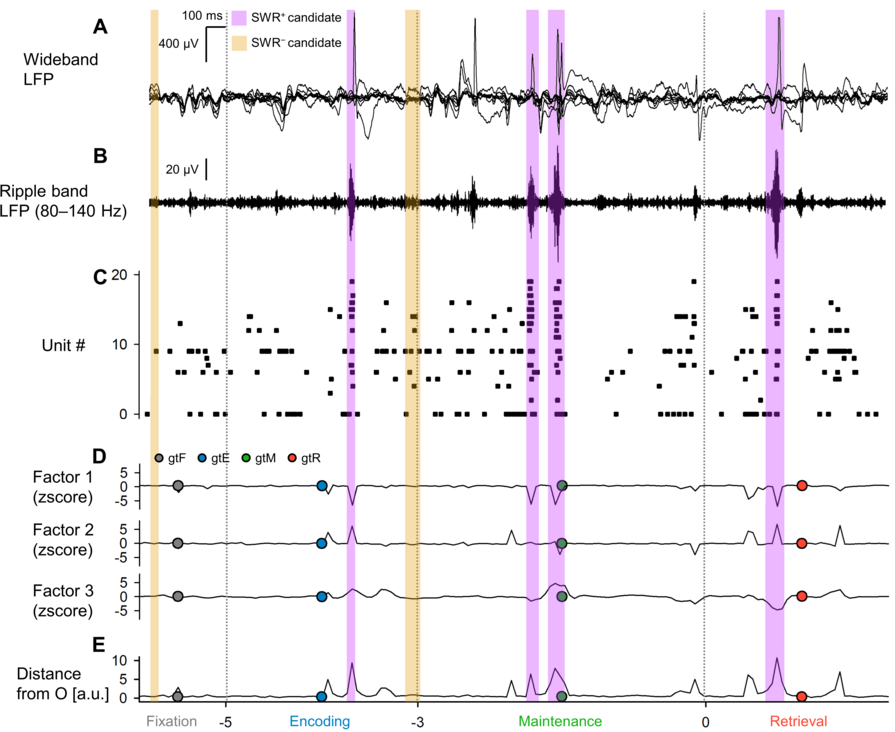
\includegraphics[width=1\textwidth]{./src/figures/.png/Figure_ID_01.png}
        	\caption{\textbf{
Local Field Potentials (LFP), Multiunit Activity, and Neural Trajectories in the Hippocampus During a Modified Sternberg Task
}
\smallskip
\\
\textbf{\textit{A.}} Representative wideband LFP signals for intracranial EEG recording from the left hippocampal head are presented. This recording took place while the subject performed a modified Sternberg working memory task. Task stages included fixation (1 s, \textit{gray}), encoding (2 s, \textit{blue}), maintenance (3 s, \textit{green}), and retrieval (2 s, \textit{red}). \textbf{\textit{B.}} Displays the associated ripple band LFP traces. Note \textit{purple} and \textit{yellow} rectangles, which denote the timings for SWR$^+$ candidates and SWR$^-$ candidates, respectively (the latter serving as control events for SWR$^+$). \textbf{\textit{C.}} A raster plot illustrates multiunit spikes from the LFP traces. These spikes have been sorted using a spike algorithm \cite{niediek_reliable_2016}. \textbf{\textit{D.}} Shows neural trajectories computed by GPFA\cite{yu_gaussian-process_2009} based on spike counts per unit with 50-ms bins. The geometric median of each phase is marked by dot circles. \textbf{\textit{E.}} Indicates the distance of the neural trajectory from the origin point $O$.
}
% width=1\textwidth
        	\label{fig:01}
        \end{figure*}
        \clearpage
        \begin{figure*}[ht]
            \pdfbookmark[2]{ID 02}{figure_id_02}
        	\centering
            \includegraphics[width=0.5\textwidth]{./src/figures/.png/Figure_ID_02.png}
        	\caption{\textbf{
State-Dependent Trajectories of Hippocampal Neurons
}
\smallskip
\\
\textbf{\textit{A.}} Neural trajectories are depicted as a point cloud within the first three-dimensional factors derived from GPFA \cite{yu_gaussian-process_2009}. The smaller dots represent 50-ms neural trajectory bins, and the larger dots with \textit{black} edges denote the geometric medians for each phase in the Sternberg working memory task: fixation ($\mathrm{\lVert g_{F} \rVert}$, \textit{gray}), encoding ($\mathrm{\lVert g_{E} \rVert}$, \textit{blue}), maintenance ($\mathrm{\lVert g_{M} \rVert}$, \textit{green}), and retrieval ($\mathrm{\lVert g_{R} \rVert}$, \textit{red}). \textbf{\textit{B.}} The figure presents the log-likelihood of the GPFA models versus the number of dimensions used to embed multiunit spikes found in the medial temporal lobe (MTL) regions. Specifically, the elbow method identified three as the optimal dimension. \textbf{\textit{C.}} This panel displays the distance of the neural trajectories from the origin ($O$) for the hippocampus (Hipp.), entorhinal cortex (EC), and amygdala (Amy.), plotted against the time elapsed from the probe onset. \textbf{\textit{D.}} The trajectory distance from $O$ within the MTL regions is shown. The hippocampus has the greatest distance, followed by the EC and the Amygdala. \textbf{\textit{E.}} The box plot illustrates inter-phase trajectory distances within the MTL regions.
}
% width=0.5\textwidth
        	\label{fig:02}
        \end{figure*}
        \clearpage
        \begin{figure*}[ht]
            \pdfbookmark[2]{ID 03}{figure_id_03}
        	\centering
            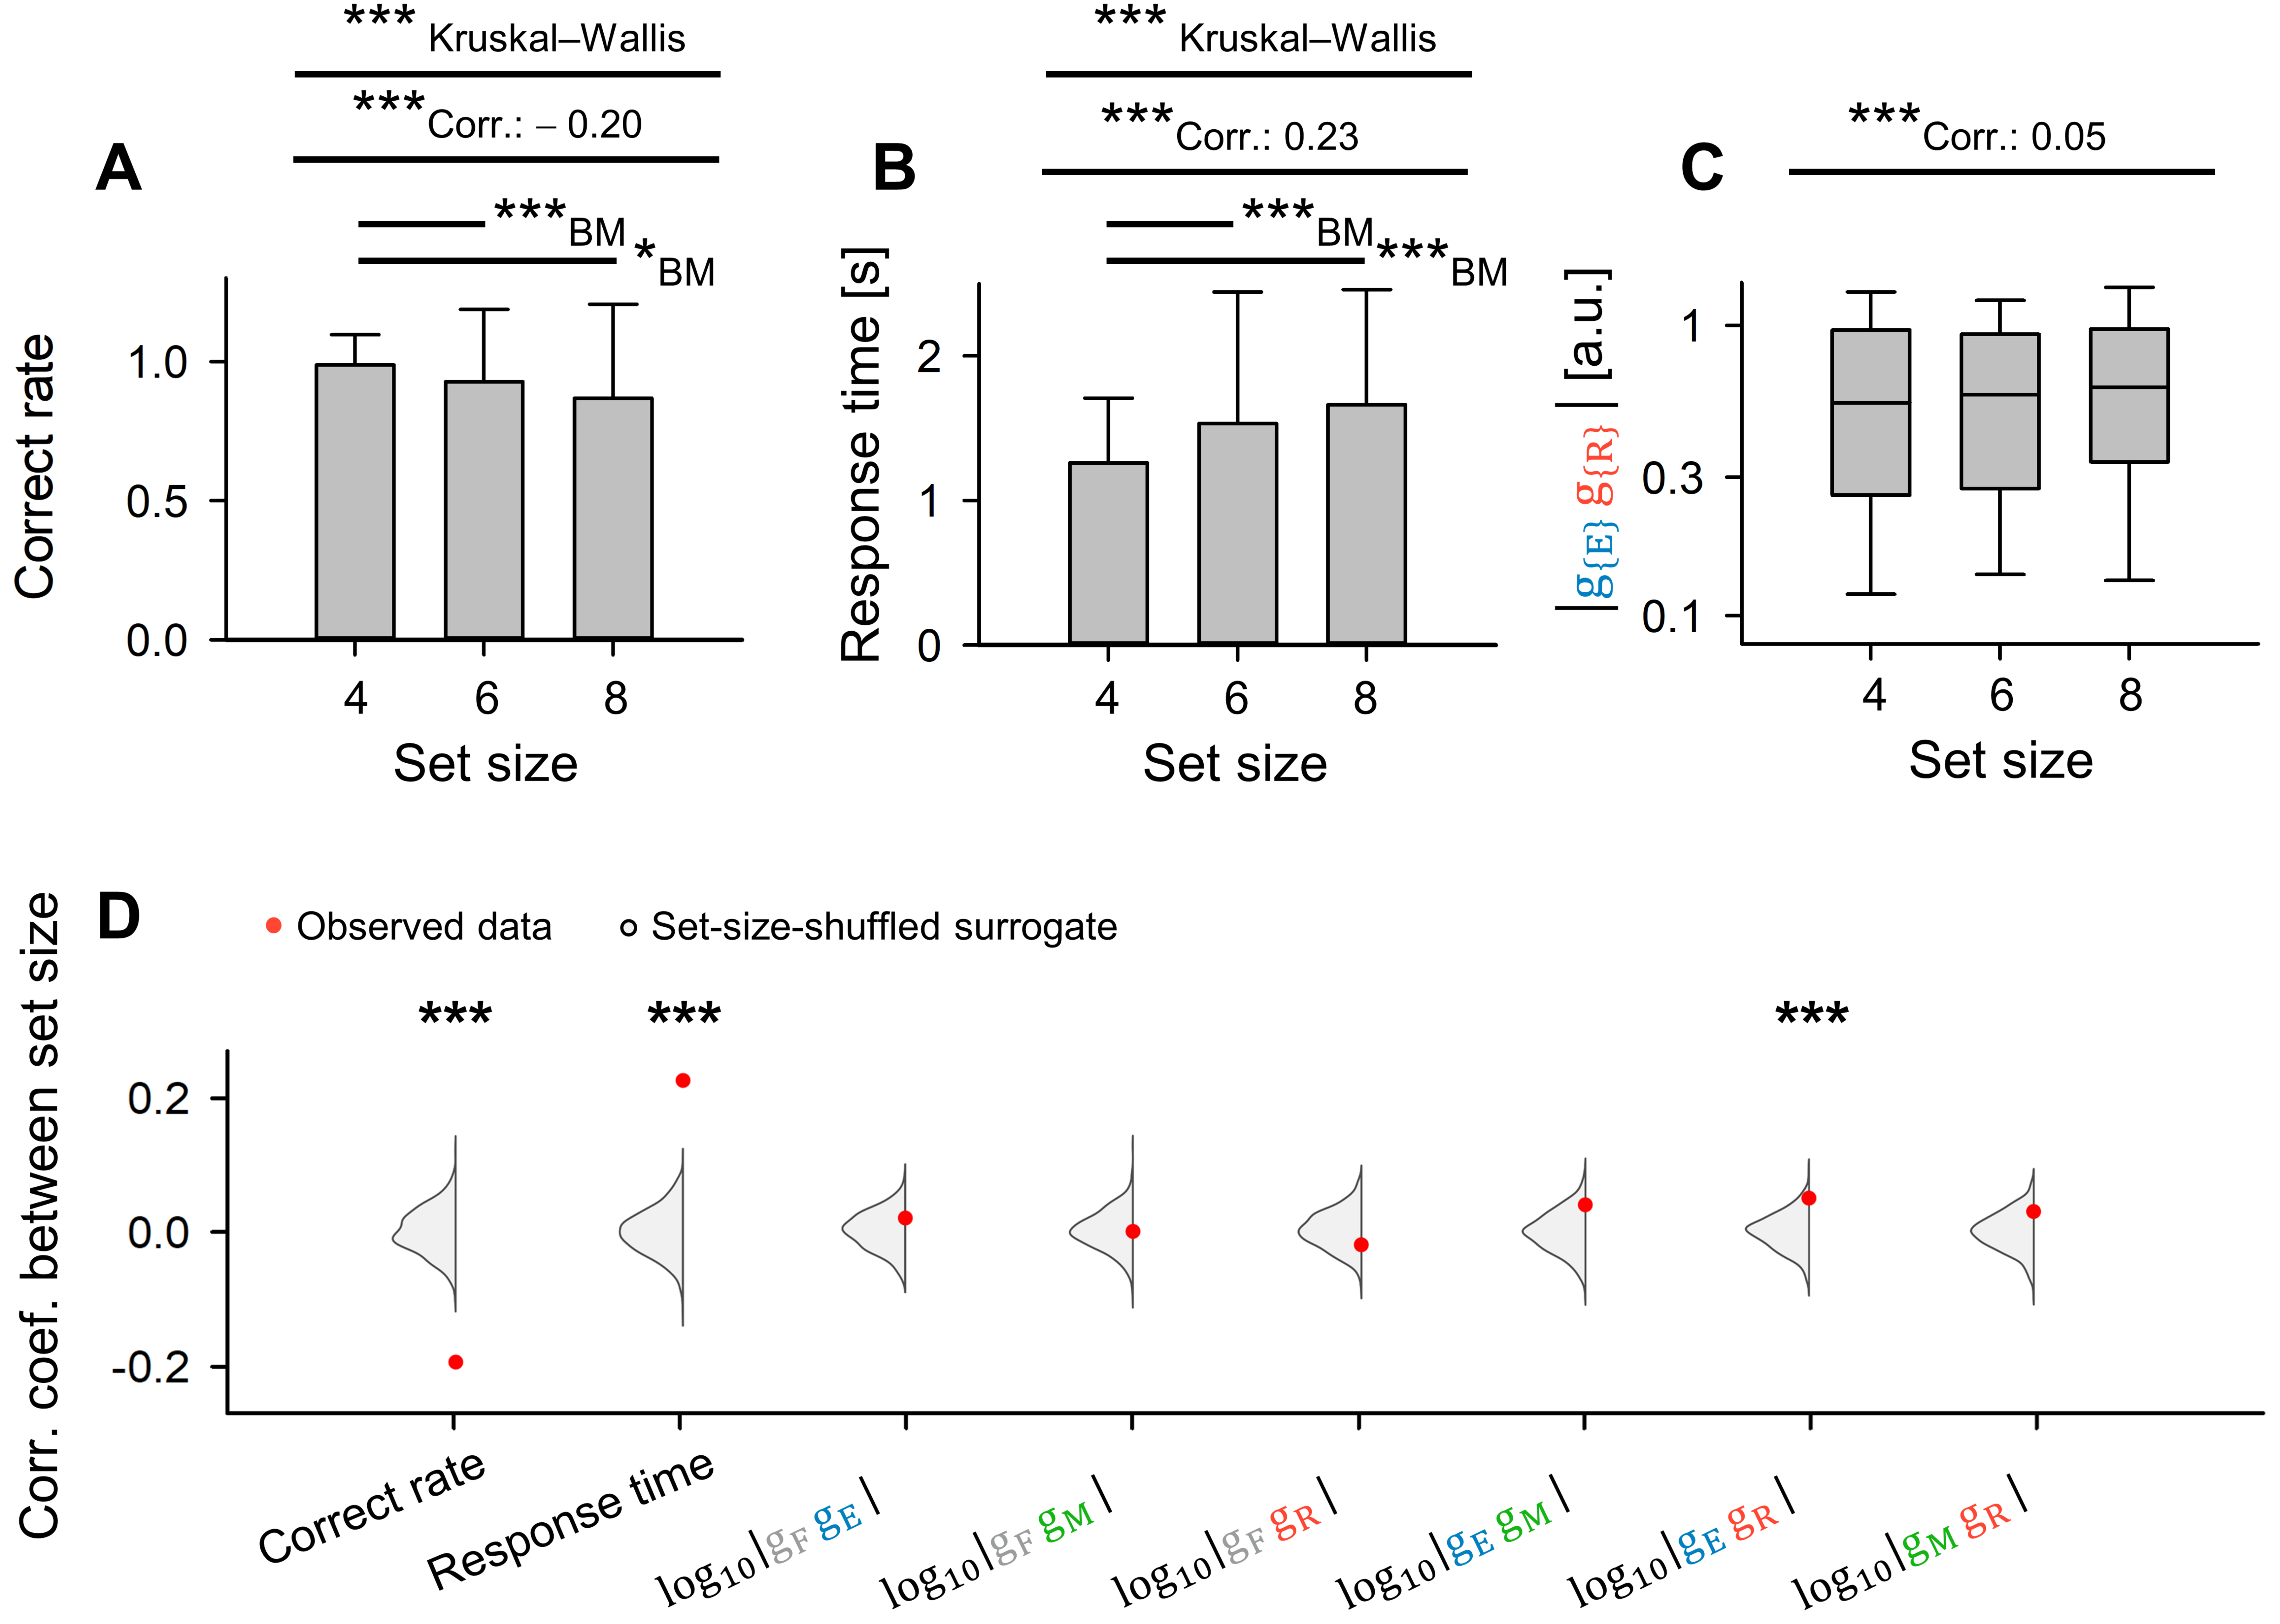
\includegraphics[width=1\textwidth]{./src/figures/.png/Figure_ID_03.png}
        	\caption{\textbf{
Relationship between Trajectory Distance and Memory Load: States of Encoding and Retrieval in the Hippocampus
}
\smallskip
\\
\textbf{\textit{A.}} Demonstrates the relationship between set size (number of letters to be encoded) and accuracy in the working memory task (coefficient = $-0.20$, ***\textit{p} $<$ 0.001). \textbf{\textit{B.}} Displays the correlation between set size and response time (coefficient = 0.23, ***\textit{p} $<$ 0.001). \textbf{\textit{C.}} Exhibits the influence of set size on the inter-phase distances between the encoding and retrieval phases ($\lVert \mathrm{g_{E}g_{R}} \rVert$) (correlation coefficient = 0.05, ***\textit{p} $<$ 0.001). \textbf{\textit{D.}} Indicates experimental observations of correlations between set size and the following parameters: accuracy, response time, $\log_{10}{\lVert \mathrm{g_{F}g_{E}} \rVert}$, $\log_{10}{\lVert \mathrm{g_{F}g_{M}} \rVert}$, $\log_{10}{\lVert \mathrm{g_{F}g_{R}} \rVert}$, $\log_{10}{\lVert \mathrm{g_{E}g_{M}} \rVert}$, $\log_{10}{\lVert \mathrm{g_{E}g_{R}} \rVert}$, and $\log_{10}{\lVert \mathrm{g_{M}g_{R}} \rVert}$ represented by \textit{red} dots. The \textit{gray} kernel density plots illustrate the corresponding shuffled surrogate with set size (\textit{n} = 1,000) (***\textit{p}s $<$ 0.001).
}
% width=1\textwidth
        	\label{fig:03}
        \end{figure*}
        \clearpage
        \begin{figure*}[ht]
            \pdfbookmark[2]{ID 04}{figure_id_04}
        	\centering
            \DIFdelbeginFL %DIFDELCMD < \includegraphics[width=]{./src/figures/.png/Figure_ID_04.png}
%DIFDELCMD <         	%%%
\DIFdelendFL \DIFaddbeginFL \includegraphics[width=1\textwidth]{./src/figures/.png/Figure_ID_04.png}
        	\DIFaddendFL \caption{\DIFdelbeginFL \textbf{\DIFdelFL{Detection of SWRs in Presumptive CA1 Regions}}%DIFAUXCMD
\DIFdelendFL \DIFaddbeginFL \textbf{\DIFaddFL{Detection of SWRs in Putative CA1 Regions}}\DIFaddendFL \\
\textbf{\textit{A.}} Two-dimensional UMAP \cite{mcinnes_umap_2018} projection displays multi-unit spikes during SWR$^+$ candidates (\textit{purple}) and SWR$^-$ candidates (\textit{yellow}). \textbf{\textit{B.}} A cumulative density plot indicates silhouette scores, reflecting UMAP clustering quality (see Table~\ref{tab:02}). Hippocampal regions with silhouette scores exceeding 0.60 (equivalent to the $75^{th}$ percentile) are identified as putative CA1 regions. SWR$^+$ and SWR$^-$ candidates, which were recorded from these regions, are classified as SWR$^+$ and SWR$^-$ respectively (\textit{n}s = 1,170). \textbf{\textit{C.}} Identical distributions of durations are presented for SWR$^+$ (\textit{purple}) and SWR$^-$ (\textit{yellow}), based on their definitions (93.0 [65.4] ms, median [IQR]). \textbf{\textit{D.}} SWR incidence for both SWR$^+$ (\textit{purple}) and SWR$^-$ (\textit{yellow}), relative to the probe's timing, is illustrated as a mean \textpm 95\% confidence interval. However, intervals may not be visibly apparent due to their confined ranges, be aware that a significant SWR incidence increase was detected during the initial 400 ms of the retrieval phase (0.421 [Hz], *\textit{p} $<$ 0.05, bootstrap test). \textbf{\textit{E.}} Distributions of ripple band peak amplitudes for SWR$^-$ (\textit{yellow}; 2.37 [0.33] SD of baseline, median [IQR]) and SWR$^+$ (\textit{purple}; 3.05 [0.85] SD of baseline, median [IQR]) are manifested (***\textit{p} $<$ 0.001, the Brunner--Munzel test).}
%DIF >  width=1\textwidth
        	\label{fig:04}
        \end{figure*}
        \clearpage
        \begin{figure*}[ht]
            \pdfbookmark[2]{ID 05}{figure_id_05}
        	\centering
            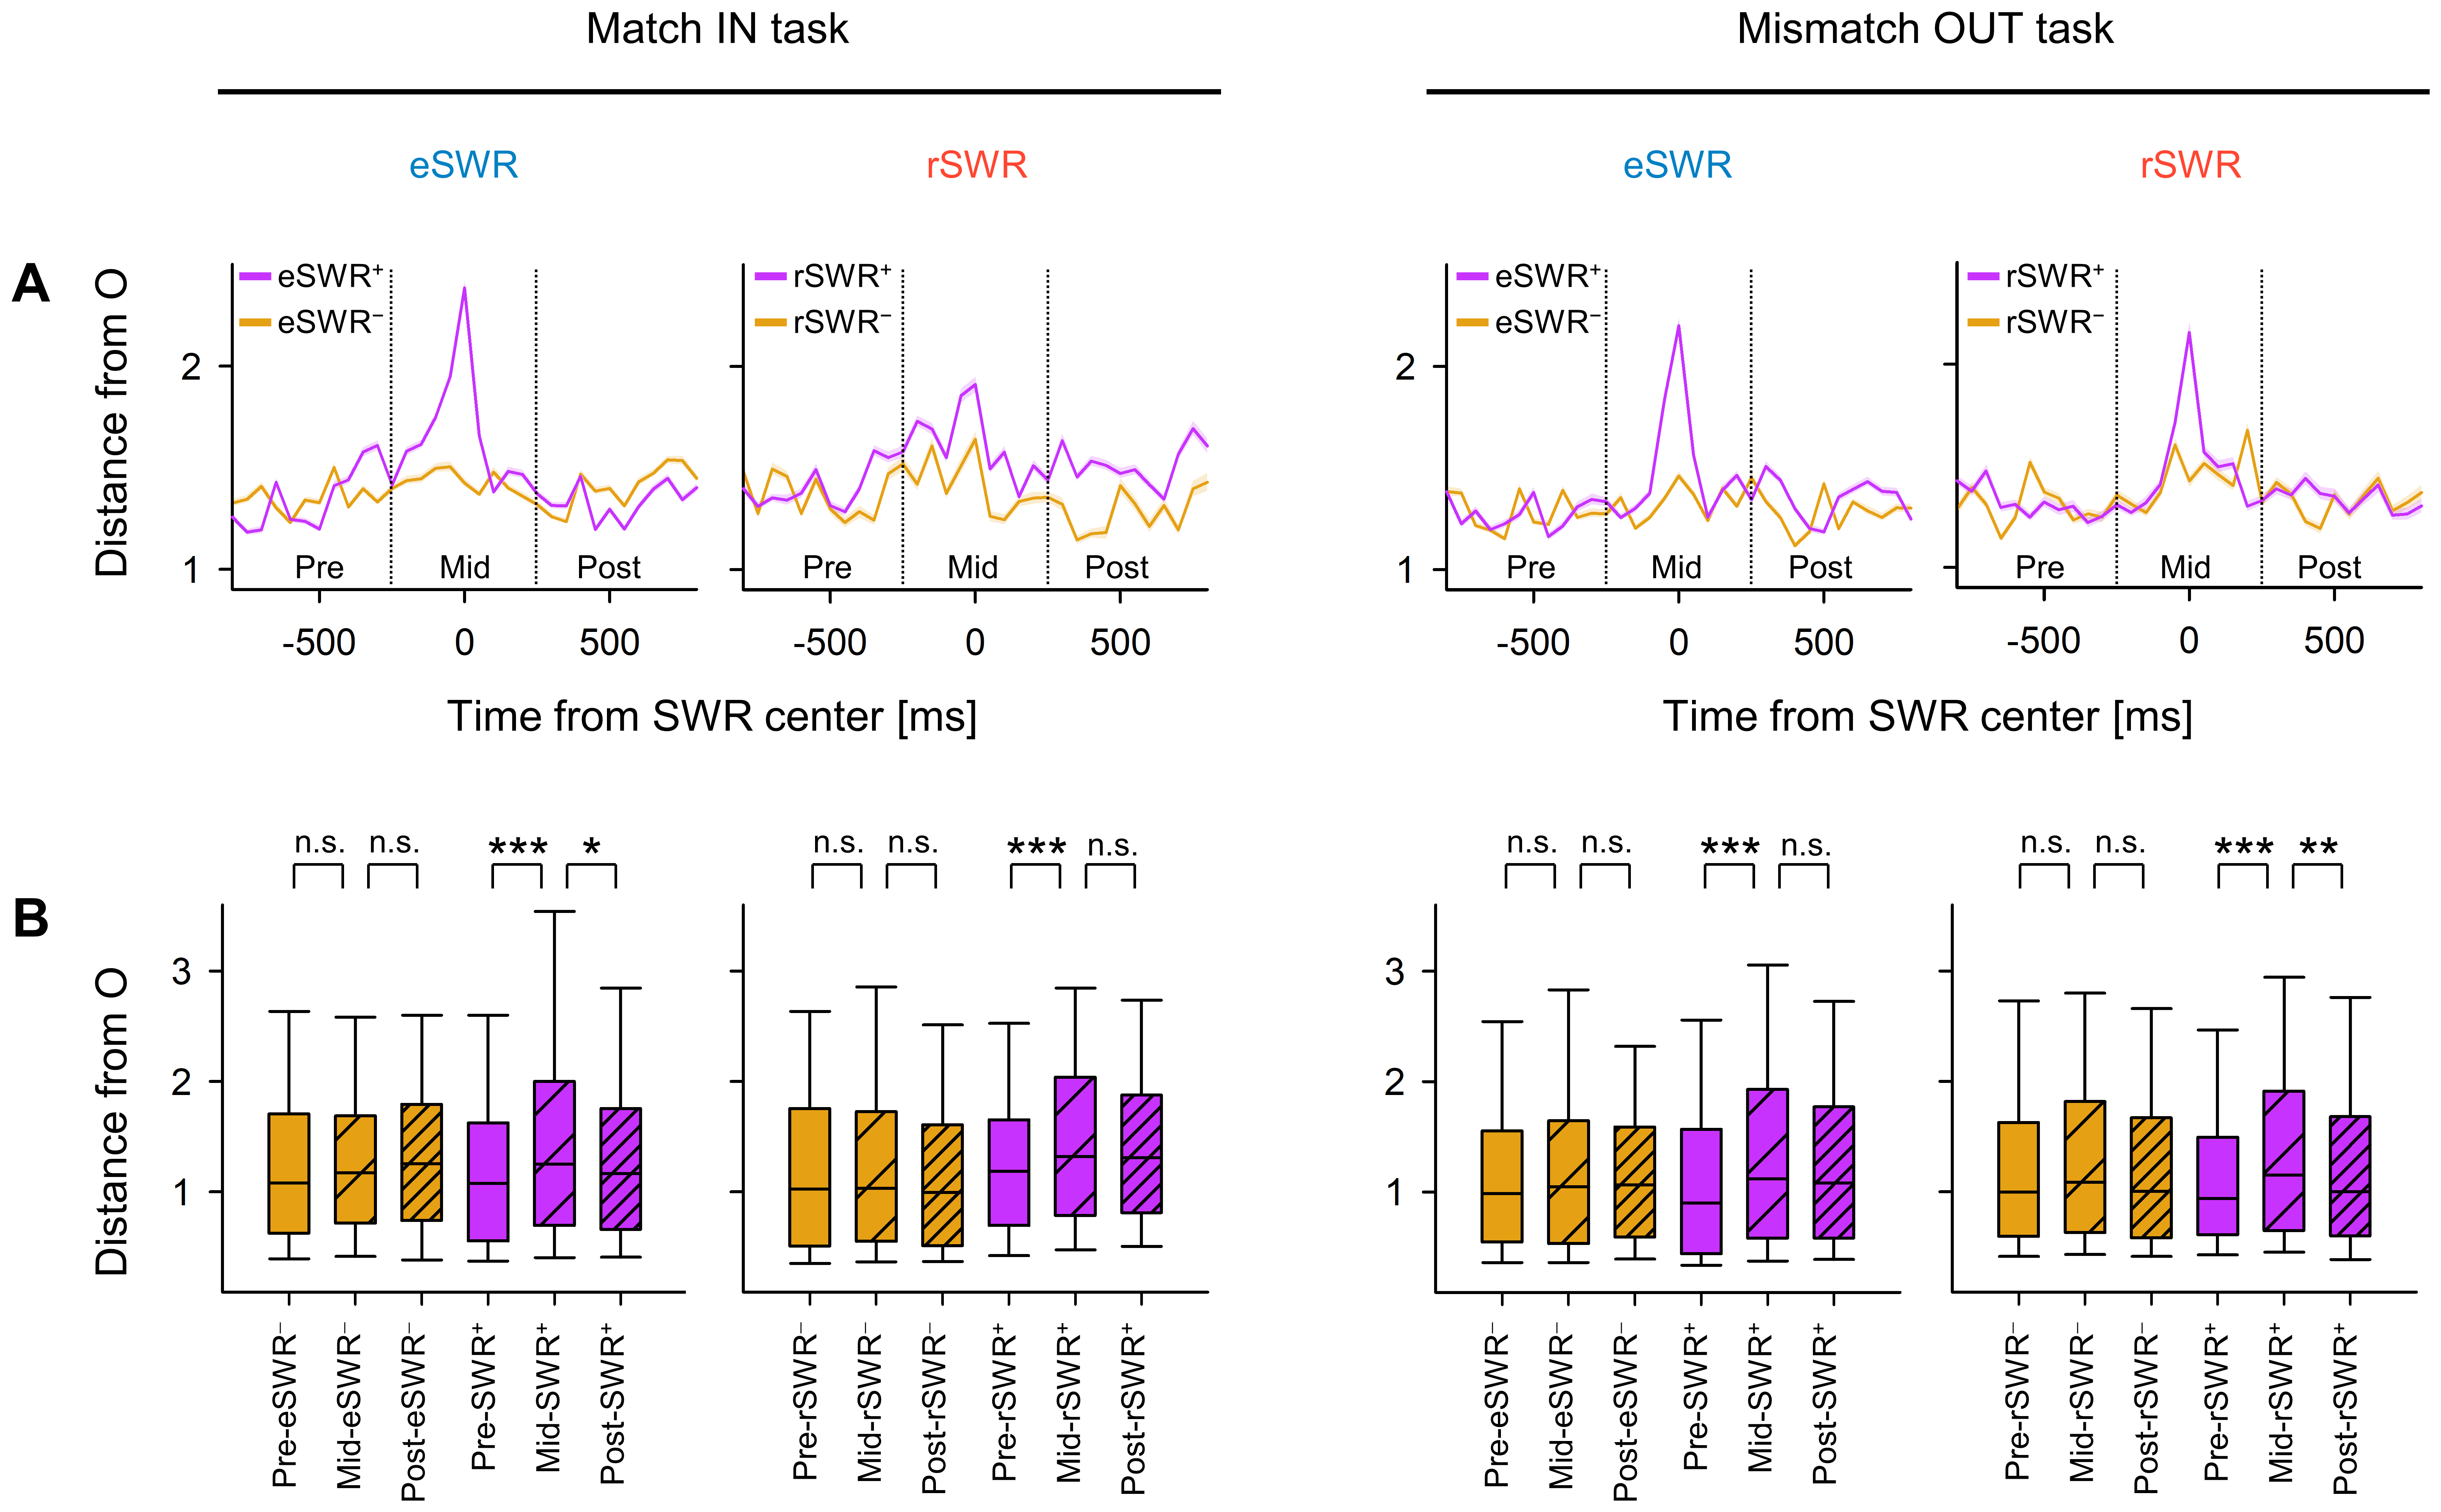
\includegraphics[width=1\textwidth]{./src/figures/.png/Figure_ID_05.png}
        	\caption{\textbf{Transient Changes in Neural Pathway During SWR Events}
\smallskip
\\
\textbf{\textit{A.}} Presented is the distance from origin ($O$) of the peri-sharp-wave-ripple pathway (mean \textpm 95\% confidence interval). The intervals may be obscured due to their minimal ranges. \textbf{\textit{B.}} The distance from the origin ($O$) during the pre-, mid-, and post-SWR periods is demonstrated (*\textit{p} $<$ 0.05, **\textit{p} $<$ 0.01, ***\textit{p} $<$ 0.001; Brunner--Munzel test applied). Abbreviations: SWR, sharp-wave ripple events; eSWR, SWR during the encoding phase; rSWR, SWR within the retrieval phase; SWR$^+$, positive SWR event; SWR$^-$, control events for SWR$^+$; pre-, mid-, or post-SWR refer to the time intervals from $-800$ to $-250$ ms, from $-250$ to $+250$ ms, or from $+250$ to $+800$ ms, respectively, all relative to the SWR center.}
% width=1\textwidth
        	\label{fig:05}
        \end{figure*}
        \clearpage
        \begin{figure*}[ht]
            \pdfbookmark[2]{ID 06}{figure_id_06}
        	\centering
            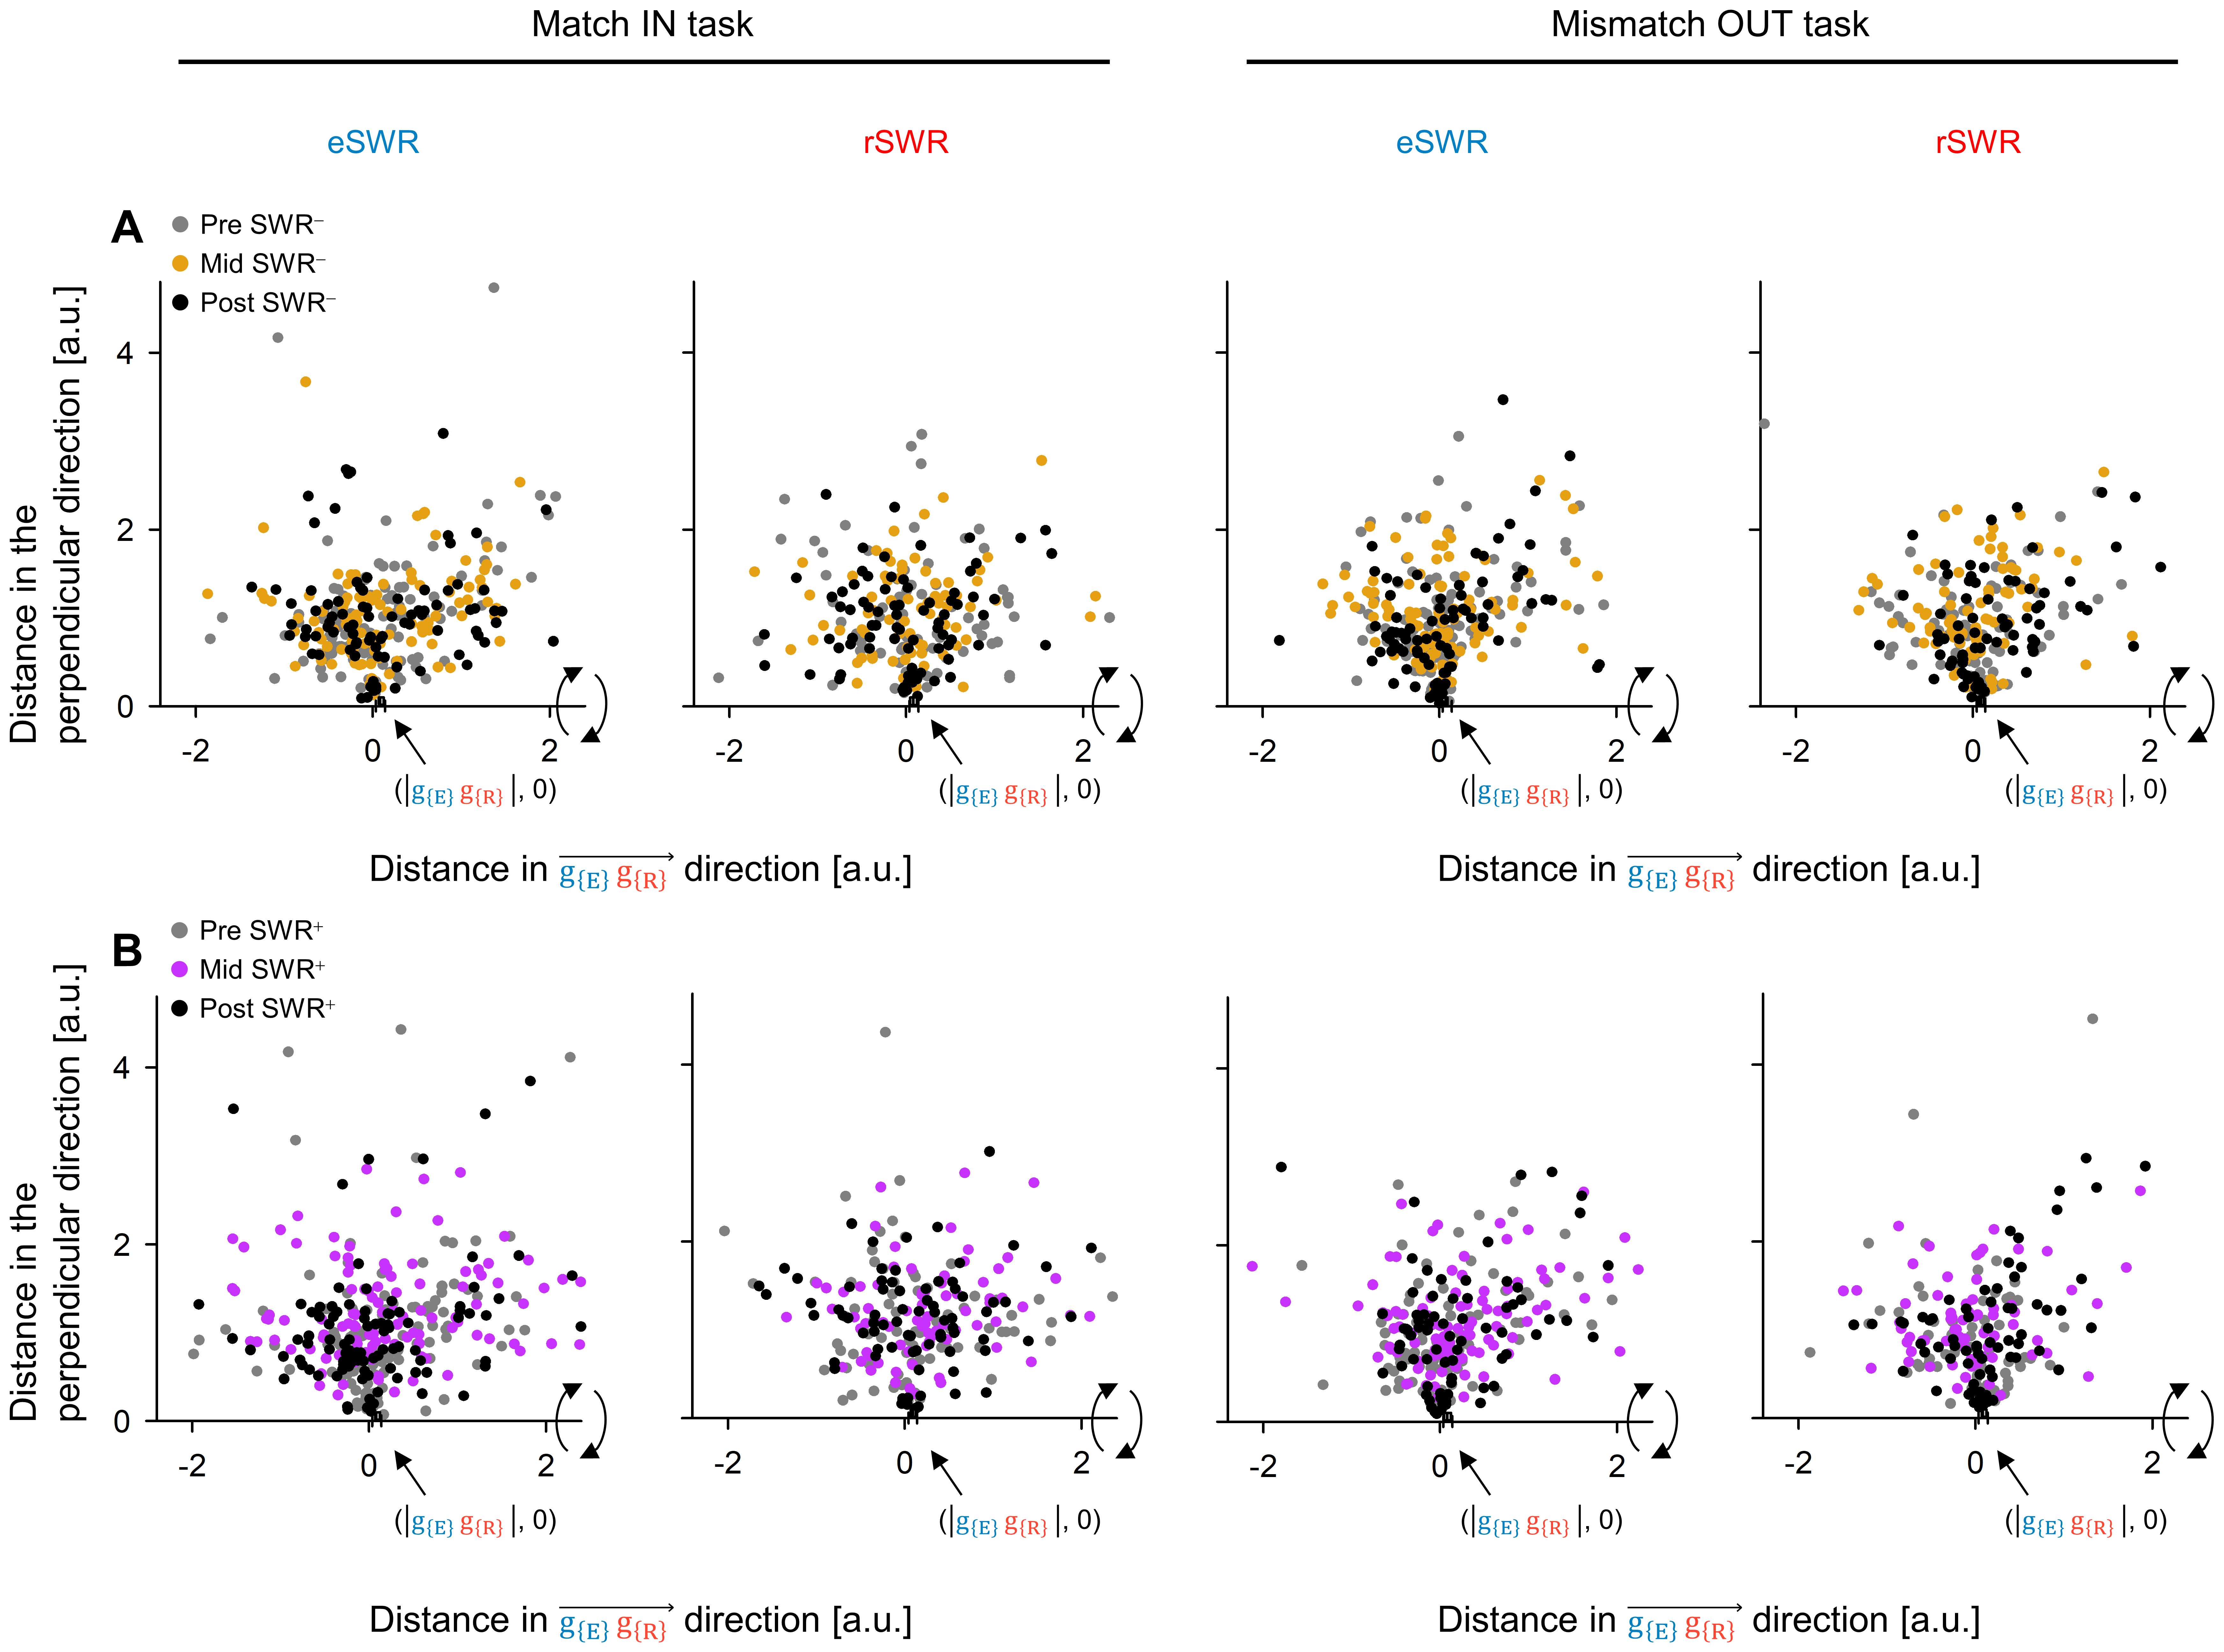
\includegraphics[width=1\textwidth]{./src/figures/.png/Figure_ID_06.png}
        	\caption{\textbf{
Visualization of Neural Trajectories during SWR in Two-Dimensional Spaces}
\smallskip
\\
The panels depict hippocampal neural trajectories during SWR projected onto two-dimensional spaces. \textbf{\textit{A.}} Shows the hippocampal neural trajectories as point clouds during pre-SWR$^-$ (\textit{gray}), mid-SWR$^-$ (\textit{yellow}), and post-SWR$^-$ (\textit{black}). \textbf{\textit{B.}} Conveys the equivalent for SWR$^+$ rather than SWR$^-$. The projection was executed as follows: First, a linear transformation placed $\mathrm{g_{E}}$ at the origin $O$ (0,0), and $\mathrm{g_{R}}$ at ($\lVert \mathrm{g_{E}g_{R}} \rVert$, 0). The point cloud was subsequently rotated around the $\mathrm{g_{E}g_{R}}$ axis (similar to the x axis) for adaptation to two-dimensional spaces. Thus, within these two-dimensional spaces, the distances from point $O$ and the angles for the $\mathrm{g_{E}g_{R}}$ axis are retained as in the original three-dimensional spaces created by GPFA. Abbreviations: SWR denotes sharp-wave ripple events; eSWR refers to SWR during the encoding phase; rSWR signals SWR during the retrieval phase; SWR$^+$, characterizes an SWR event; SWR$^-$ signifies control events for SWR$^+$; pre-SWR, mid-SWR, or post-SWR, represent the time intervals from $-800$ to $-250$ ms, from $-250$ to $+250$ ms, or from $+250$ to $+800$ ms from the center of the SWR.
}
% width=1\textwidth
        	\label{fig:06}
        \end{figure*}
        \clearpage
        \begin{figure*}[ht]
            \pdfbookmark[2]{ID 07}{figure_id_07}
        	\centering
            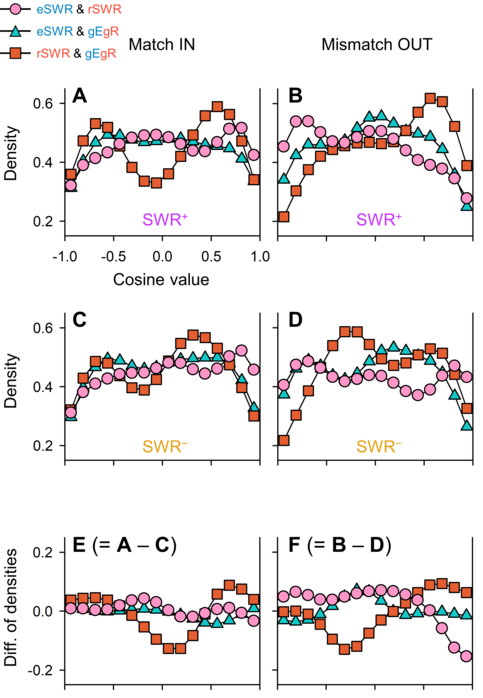
\includegraphics[width=0.5\textwidth]{./src/figures/.png/Figure_ID_07.png}
        	\caption{\textbf{
Neural Trajectories Direction during SWRs Based on Encoding and Retrieval States
}
\smallskip
\\
\textbf{\textit{A--B}} Shows the kernel density estimation distributions of $\protect\overrightarrow{{\mathrm{eSWR^+}}}$ $\cdot$ $\protect\overrightarrow{{\mathrm{rSWR^+}}}$ (depicted as pink circles), $\protect\overrightarrow{{\mathrm{eSWR^+}}}$ $\cdot$ $\protect\overrightarrow{{\mathrm{g_{E}g_{R}}}}$ (blue triangles), and $\protect\overrightarrow{{\mathrm{rSWR^+}}}$ $\cdot$ $\protect\overrightarrow{{\mathrm{g_{E}g_{R}}}}$ (red rectangles) in the Match In (\textit{A}) and Mismatch OUT tasks (\textit{B}). \textbf{\textit{C--D}} Illustrates the corresponding distributions of $\mathrm{SWR^-}$ instead of those of $\mathrm{SWR^+}$ in \textit{A} and \textit{B}. \textbf{\textit{E--F}} Renders the differences in the distributions of $\mathrm{SWR^+}$ and $\mathrm{SWR^-}$, detailing the SWR components (\textit{E} = \textit{C} - \textit{A} & \textit{F} = \textit{D} - \textit{B}). The biphasic distributions of $\protect\overrightarrow{{\mathrm{rSWR^-}}}$ $\cdot$ $\protect\overrightarrow{{\mathrm{g_{E}g_{R}}}}$ indicates fluctuations between the encoding and retrieval states during the Sternberg task. Also, contradicting directionality between $\protect\overrightarrow{{\mathrm{eSWR^+}}}$ and $\protect\overrightarrow{{\mathrm{rSWR^+}}}$ was observed (pink circles) not in the Match IN task (\textbf{\textit{E}}), but in Mismatch OUT task (\textbf{\textit{F}}). Lastly, transition from the retrieval to encoding states are apparent in the SWR components in both Match IN and Mismatch OUT tasks (red rectangles in \textit{E--F}).
}
% width=0.5\textwidth
        	\label{fig:07}
        \end{figure*}

%%%%%%%%%%%%%%%%%%%%%%%%%%%%%%%%%%%%%%%%%%%%%%%%%%%%%%%%%%%%%%%%%%%%%%%%%%%%%%%%
%% END
%%%%%%%%%%%%%%%%%%%%%%%%%%%%%%%%%%%%%%%%%%%%%%%%%%%%%%%%%%%%%%%%%%%%%%%%%%%%%%%%

\end{document}
